% Chapter 11: Worked example
\chapter{Worked Example}\label{chap:11}
\label{ch:11}

This chapter goes through a complete study with two built-in case studies:
\begin{itemize}
  \item \textbf{Part A, BBD extraction} (\ui{Extraction Optimization (Box-Behnken)}): a designed experiment with 17
        runs and two conflicting responses. It is used for the whole route from data to confirmation: readiness, RSM,
        ANN, desirability, NSGA-II, the checks C and D, sensitivity and prediction.
  \item \textbf{Part B, dye adsorption} (\ui{Dye Adsorption (ANN, 40 runs)}): 40 historical runs of a strongly nonlinear
        process with one response. It shows when an ANN is justified, with the checks A and B.
  \item \textbf{Part C, polygeneration plant} (\ui{Polygeneration Plant (3 Objectives)}): 80 simulated runs of an
        illustrative plant model with five decision variables and three conflicting objectives. It is a complete
        multi-objective study: readiness, RSM and ANN with checks A and B, NSGA-III with checks C and D, sensitivity,
        choice of the compromise, confirmation plan and export (Section~\ref{sec:ch11-polygen}). A short note on the
        mixture variant (\ui{Concrete Mix Paste (Mixture, 3 Objectives)}) closes the part.
\end{itemize}
All numbers below are those of the screenshots of this manual: design seed 12345, ANN seed 1, NSGA seed 1, one CPU
core. If you repeat the steps with the same settings you should see the same values; on a different computer the last
digits of the ANN results may differ.

A note on honesty before we start: not every check passes in this example. Check~D fails for the BBD case, and the
reasons are instructive. The text explains what the failure means and what to do about it.

% ======================================================================================================
\section{Part A: open the case and check readiness}
\label{sec:ch11-open}

\subsection{Open the case study}
\begin{enumerate}
  \item Choose \menupath{File $\rightarrow$ Case Studies\dots} (or \ui{Case studies} on the start page, or
        \ui{Case Studies} on the toolbar).
  \item Select \ui{Extraction Optimization (Box-Behnken)} and click \ui{Open Case Study}
        (Figure~\ref{fig:ch11-cases}).
\end{enumerate}

\begin{figure}[htbp]
\centering
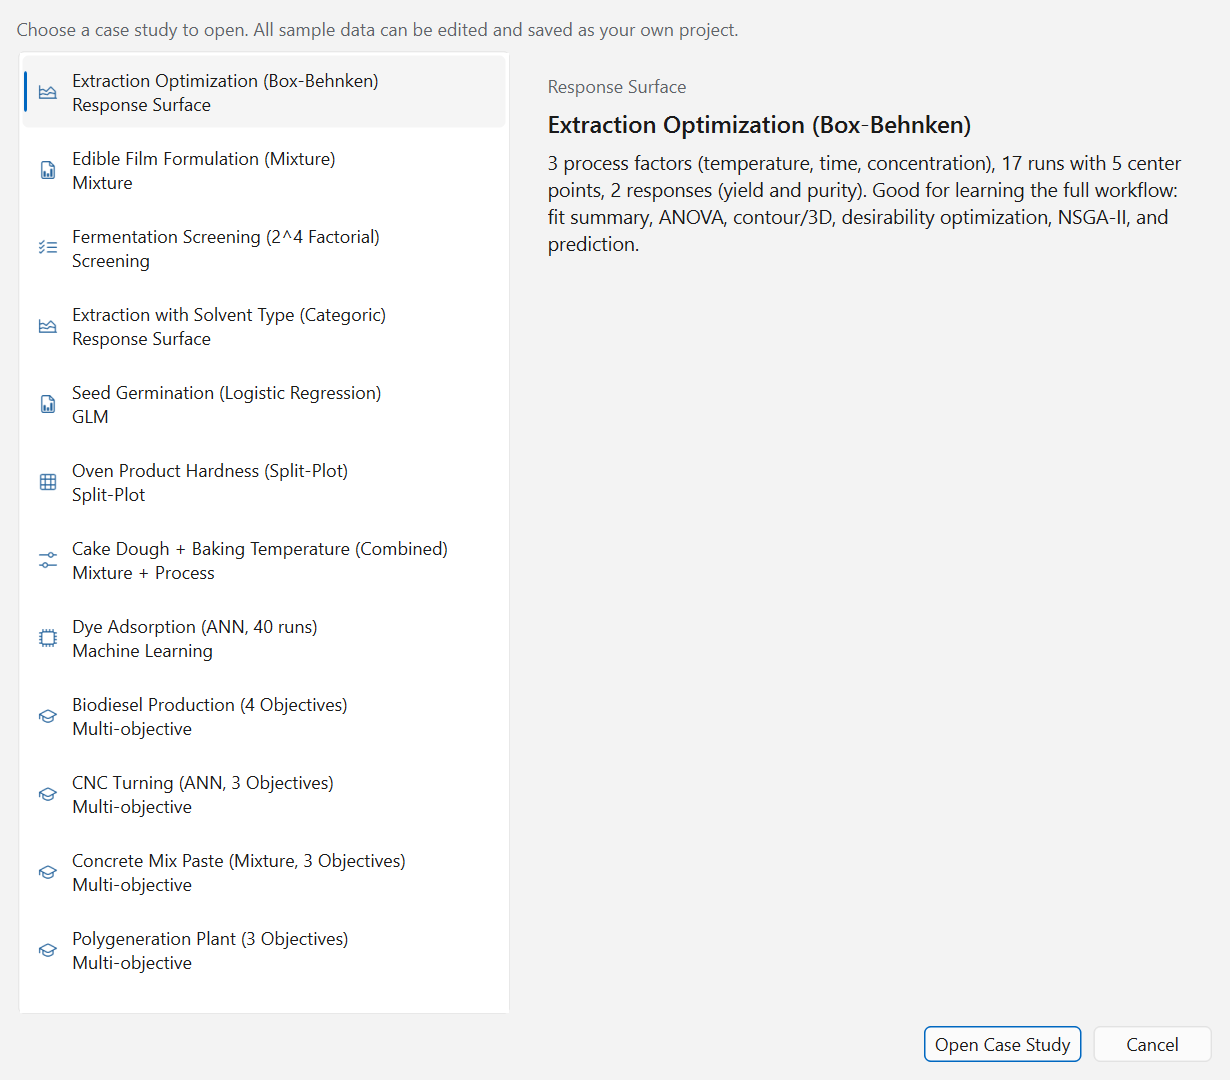
\includegraphics[width=0.75\linewidth]{case_studies.png}
\caption{The \ui{Case Studies} dialog with the BBD extraction case selected.}
\label{fig:ch11-cases}
\end{figure}

The \ui{Data} page shows a Box-Behnken design with three numeric factors, Temperature (60--80~°C), Time (30--90~min)
and Concentration (1--3~\%), 17 runs including 5 center points, and the responses Yield (\%) and Purity (\%). The goal
of the study is to maximize both.

\subsection{Data readiness}
Open \ui{Data Readiness} (Figure~\ref{fig:ch11-readiness}). With the reference model Quadratic (10 parameters) both
responses are rated \ui{Ready}: Yield scores 94 for modeling and 96 for optimization, Purity 100 and 97. The checks
behind the scores:
\begin{itemize}
  \item 17 complete runs, residual df 7, three levels per factor, pure error df 4, maximum VIF 1.01, largest gap
        in the factor space 0.27: the design is sound.
  \item Yield has two influential runs (runs 1 and 7, Cook's distance $>1$) and a significant lack of fit
        (p 0.030), both marked \ui{Needs attention}. The signal-to-noise ratio is 15.4.
  \item The optimization readiness is good: model $p=1.7\times10^{-6}$, predicted $R^2$ 0.886, the model-predicted
        maximum of Yield (75.46~°C, 86.13~min, 2.298~\%) lies inside the region, at a distance of 0.16 from the
        nearest run.
\end{itemize}
The recommendations are to check runs 1 and 7 for recording errors and, because of the lack of fit, to consider a
higher-order model, a transform or an ANN. Runs 1 and 7 belong to the design and there is no record of a problem, so
they stay in the analysis; the lack of fit is discussed below.

\begin{figure}[htbp]
\centering
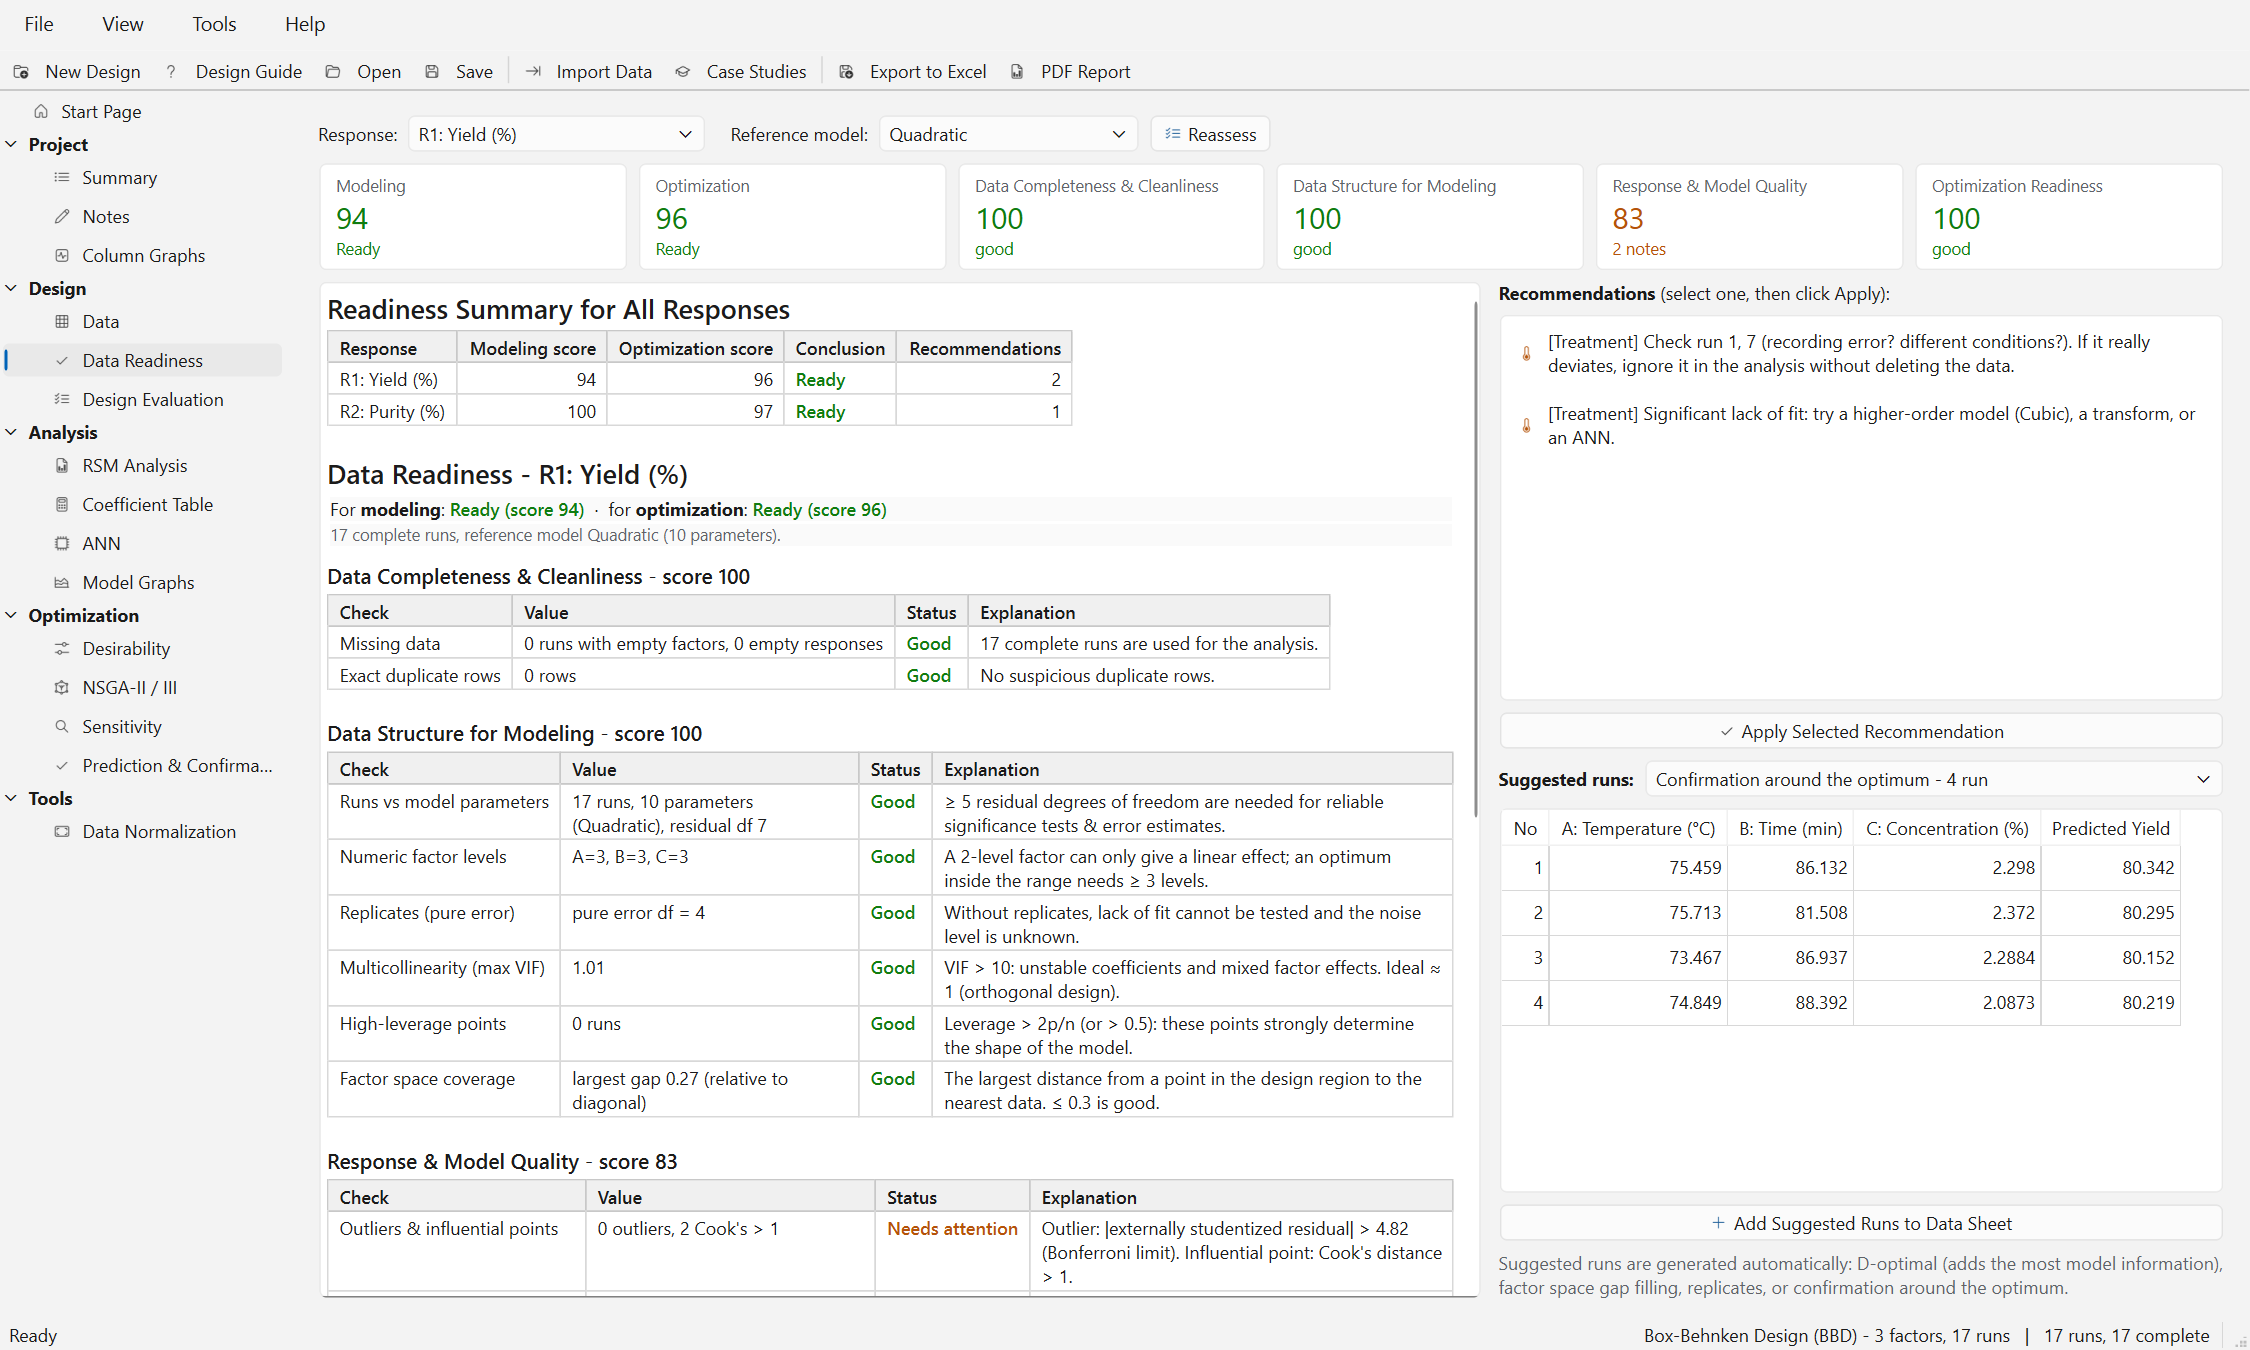
\includegraphics[width=\linewidth]{readiness.png}
\caption{\ui{Data Readiness} of the BBD case: both responses \ui{Ready}.}
\label{fig:ch11-readiness}
\end{figure}

% ======================================================================================================
\section{Part A: fit the response surface models}
\label{sec:ch11-rsm}

\subsection{Model selection and ANOVA}
On \ui{RSM Analysis}, tab \ui{Fit Summary}, the sequential model comparison for Yield suggests the quadratic model
(sequential $p<0.0001$, adjusted $R^2$ 0.9815, predicted $R^2$ 0.8857); the cubic model is aliased in a BBD. The
page marks the suggestion with \ui{Significant lack of fit} and warns ``the suggested model (Quadratic) has significant
lack of fit (p = 0.0302)''; the lack of fit is examined with the ANOVA below. Use the suggested model (\ui{Use
Suggested Model}) for both responses.

\begin{figure}[htbp]
\centering
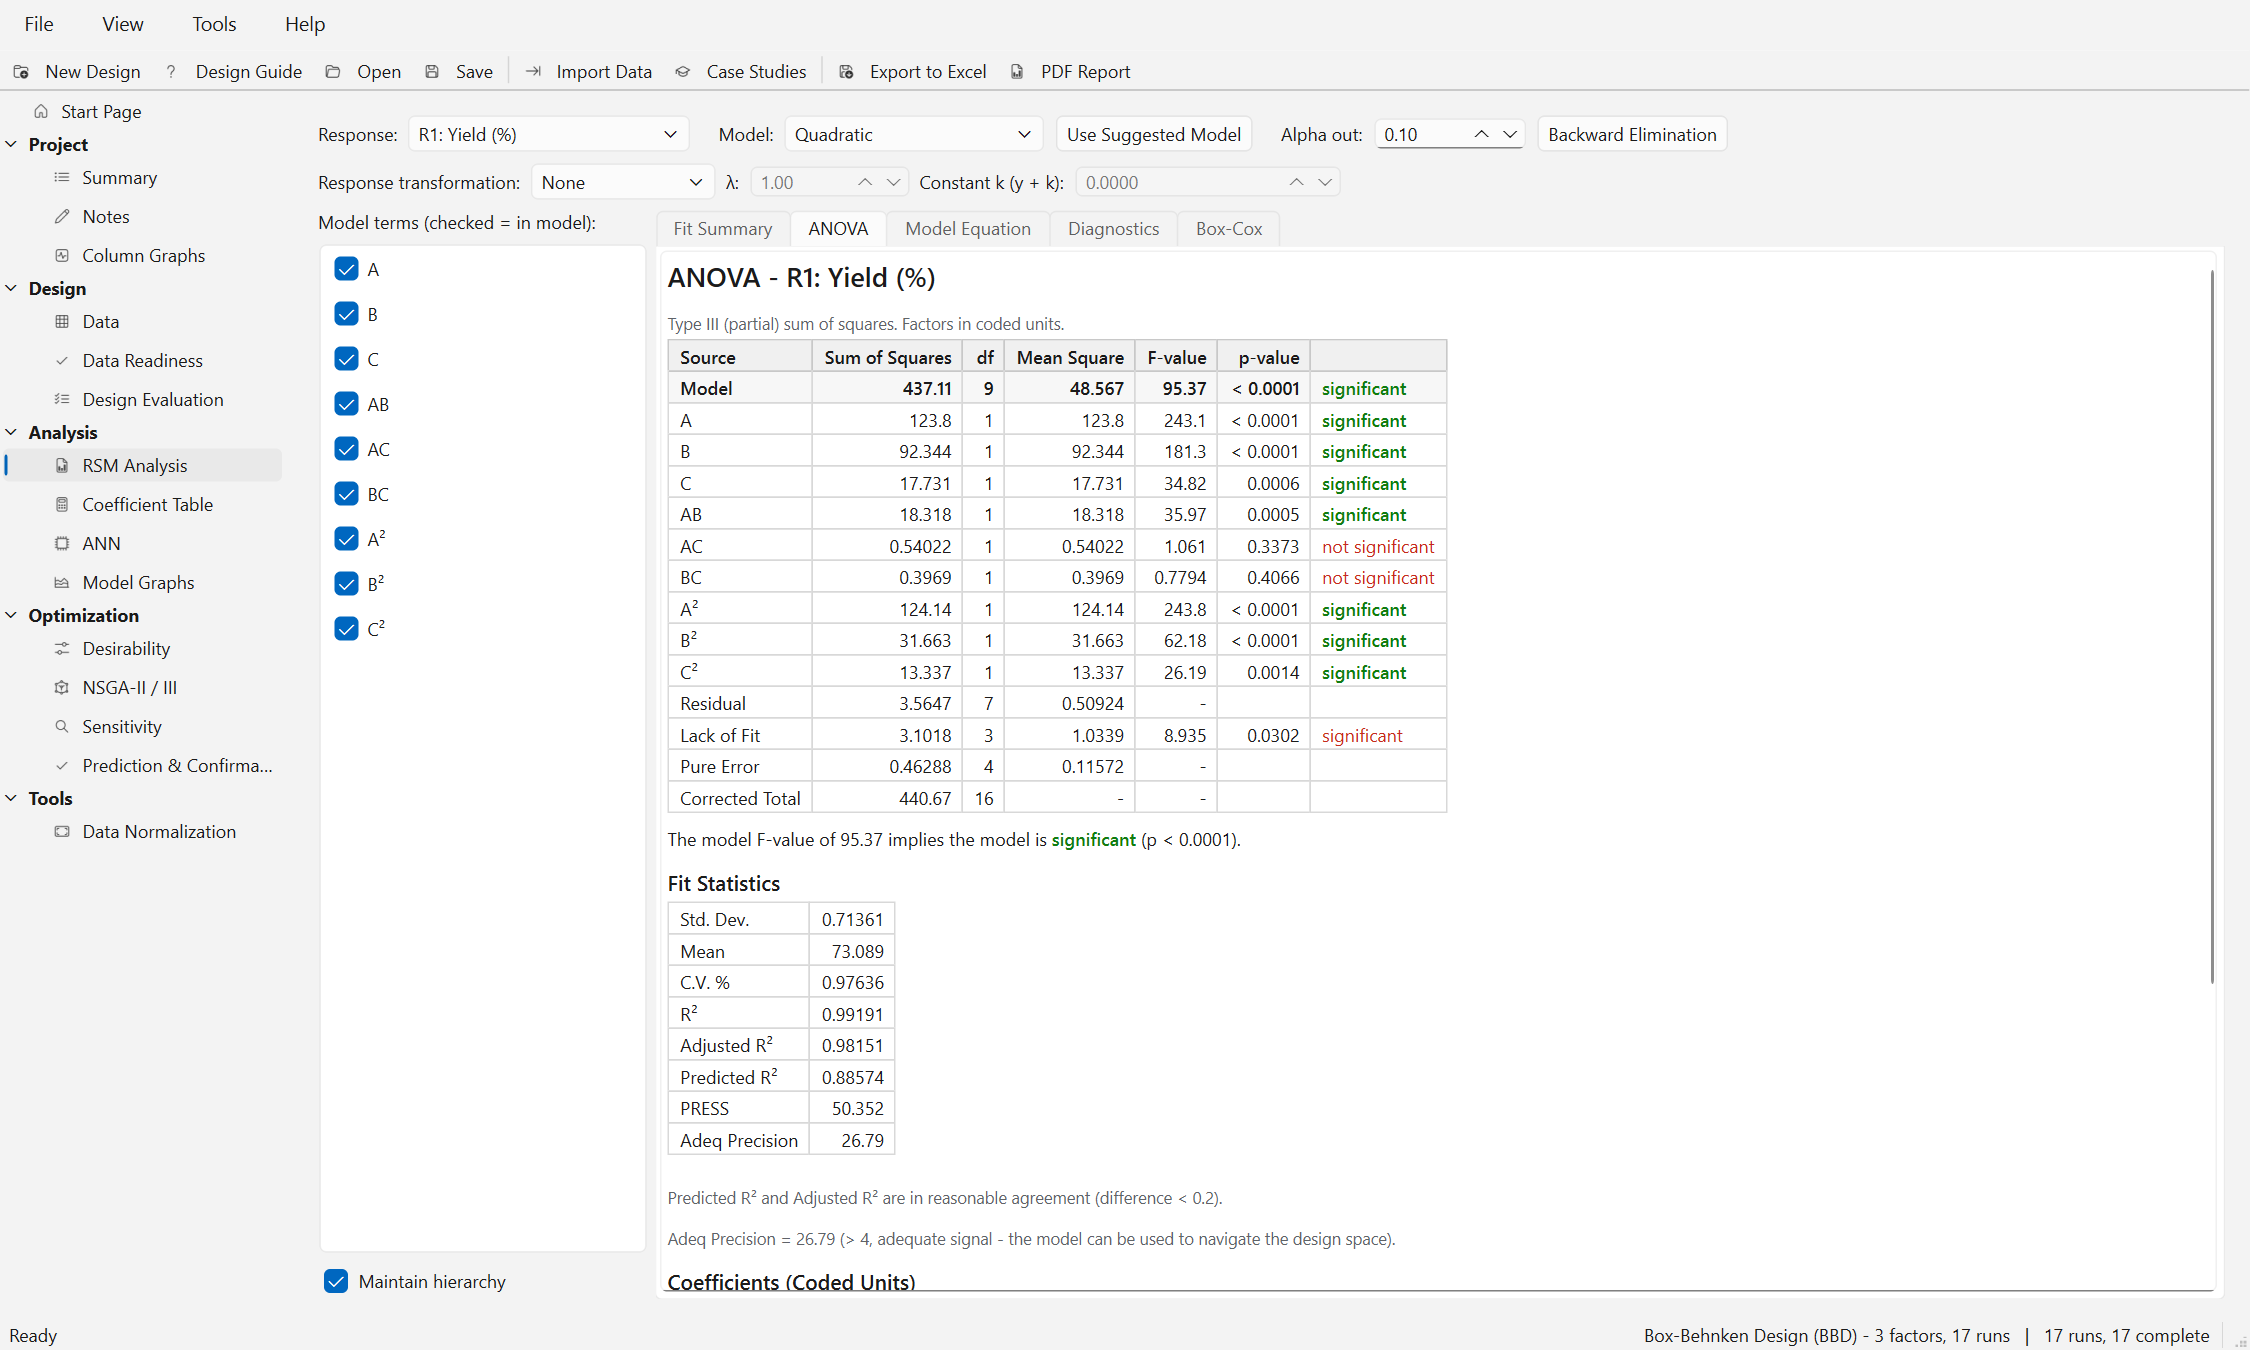
\includegraphics[width=\linewidth]{rsm_anova.png}
\caption{ANOVA of the quadratic model for Yield.}
\label{fig:ch11-anova}
\end{figure}

The \ui{ANOVA} tab for Yield (Figure~\ref{fig:ch11-anova}) gives:
\begin{itemize}
  \item Model $F=95.37$, $p<0.0001$; $R^2=0.9919$, adjusted $R^2=0.9815$, predicted $R^2=0.8857$, Adeq Precision 26.79,
        standard deviation 0.714, C.V. 0.98~\%.
  \item All linear and quadratic terms and the AB interaction are significant; AC ($p=0.337$) and BC ($p=0.407$) are
        not. Removing them would change the predictions very little; the full quadratic model is kept here so that
        both responses use the same model form.
  \item Lack of fit $F=8.935$, $p=0.0302$: significant. The pure error (mean square 0.116, 4 df from five center
        points) is very small compared with the lack-of-fit mean square (1.03). With such a precise replicate
        estimate, even small systematic deviations from the quadratic surface become significant. The lack-of-fit
        mean square corresponds to a standard deviation of about 1 percentage point of Yield, which is small relative to the response
        range (64.1--78.3), and the predicted $R^2$ of 0.886 shows that the model predicts new runs well. We accept
        the model and keep the lack of fit in mind: it is one reason to try an ANN (and to run check~D).
\end{itemize}
The equation in coded factors is
$\text{Yield}=77.772+3.934A+3.398B+1.489C+2.140AB-0.368AC-0.315BC-5.430A^2-2.742B^2-1.780C^2$.

For Purity the quadratic model gives $R^2=0.9886$, adjusted $R^2=0.974$ and predicted $R^2=0.9302$, with an
insignificant lack of fit ($p=0.638$). Temperature lowers Purity ($-2.354$ per coded unit), Time raises it.

\subsection{Diagnostics}
On \ui{Diagnostics} the normal plot of the externally studentized residuals is straight (Shapiro--Wilk $p=0.904$), no
residual exceeds the Bonferroni limit $\pm4.82$, and only runs 1 and 7 have Cook's distance above 1, the same runs as in
the readiness report. \ui{Box-Cox} recommends no transformation ($\lambda=1$ lies inside the confidence interval).
The models are adequate for optimization.

% ======================================================================================================
\section{Part A: ANN with checks A and B}
\label{sec:ch11-ann-bbd}
The lack of fit of Yield raises the question whether an ANN would do better. With 17 runs that is doubtful, and the
checks of REGEN make the answer explicit.

\begin{enumerate}
  \item Open \ui{ANN}. The \ui{Data Adequacy} report runs automatically: Yield is \ui{Adequate with caveats} (only 17
        runs, \ui{Caution}; training rows per weight 1.27, \ui{Caution}; signal/noise 15.43 and the significant lack of
        fit rate the need for a nonlinear model as \ui{Good}). Purity is \ui{Adequate with many caveats - ANN results
        need strict validation}: in addition run 8 is a response outlier (robust $z>3.5$).
  \item Set \ui{CPU cores (parallel):} to 1 if you want exactly the numbers below, leave the other settings at their
        defaults and click \ui{Optimize All Responses (One Click)}. This is \textbf{check~A}: a cross-validated
        architecture search for each response.
  \item Select each response in \ui{Show response:} and click \ui{Learning Curve (Enough Data?)}. This is
        \textbf{check~B}.
\end{enumerate}

\textbf{Check~A result.} The status line reads \ui{Done. R1: 1 layer (4) - Good fit; R2: 1 layer (5) - Good fit}.
For Yield, 26 architectures were evaluated with 5-fold cross-validation; the selected 3-4-1 network (21 weights) has a
cross-validated training $R^2$ of 0.971 and test $R^2$ ($Q^2$) of 0.624. A 3-4-5-1 network had a slightly lower test
error, but within one standard error, so the simpler network was kept (1-SE rule). 21 candidates were excluded as
overfitting. On the same folds the quadratic RSM reaches $Q^2=0.598$, so the search reports \ui{ANN predicts new data
better than RSM (assessed on the same test data)}, but the margin (0.624 against 0.598) is small. For Purity the
selected 3-5-1 network has $Q^2=0.774$, while RSM reaches 0.818: \ui{RSM predicts new data as well as or better than
ANN}.

The \ui{Summary \& Diagnosis} tab of the Yield network shows \ui{Good fit (result of 5-fold cross-validation during
architecture search)} and, as secondary information, the single train/test split of the final model (11 training,
3 validation, 3 test runs): \ui{Overfitting}, test $R^2=-0.75$. The page itself warns that 6 validation and test runs
are too few for this diagnosis; the cross-validated result is the one to use.

\textbf{Check~B result.} For both responses the learning curve ends with \ui{Learning curve finished: too little data
to assess}: \ui{Too little data (17 runs) for a reliable learning curve.} With the full data the ANN test $R^2$
(median of 10 repeats on 3 test runs) is 0.552 for Yield and 0.315 for Purity, against 0.885 and 0.911 for RSM:
\ui{RSM is more accurate at this data size}.

\textbf{Conclusion of checks A and B for Part A.} The networks are not badly overfitted, but 17 runs do not support an
ANN that is clearly better than the quadratic model. The RSM models remain the selected models (the check box
\ui{When finished, use ANN for graphs/optimization} was left off). The ANNs are kept only for check~D.

% ======================================================================================================
\section{Part A: set goals and run the desirability optimization}
\label{sec:ch11-desir}
On \ui{Desirability} set both responses to \ui{Maximize}. Raise the lower limits to the values below which a result
is of no interest, 75 for Yield and 89 for Purity; keep the upper limits at the data maxima (78.29 and 93.6), shape
1.00, importance \ui{+++} and model \ui{RSM}. Click \ui{Run Optimization}.

The result (Figure~\ref{fig:ch08-desirability} in Chapter~\ref{chap:8}) has five solutions with $D=0.845$--$0.862$. The best is
70.265~°C, 89.781~min, 1.7975~\% with predicted Yield 78.29 ($d=1$) and Purity 92.416 ($d=0.743$), $D=0.862$. Yield is
at its upper limit, so it is ``fully desirable''; all remaining freedom is used for Purity.

% ======================================================================================================
\section{Part A: NSGA-II and check C}
\label{sec:ch11-nsga}
On \ui{NSGA-II / III} the goals are already \ui{Maximize} for both responses (taken from the \ui{Desirability} page).
Keep all defaults and click \ui{Run Optimization}. Then click \ui{Check Population Size}.

\begin{itemize}
  \item The automatic algorithm choice is NSGA-II (two objectives). The run stops automatically at generation 78 with
        99 Pareto solutions (Figure~\ref{fig:ch08-front}). The front runs from Purity 94.9 at Yield 63.6 to Purity 89.6
        at Yield 80.4.
  \item TOPSIS chooses 71.527~°C, 88.239~min, 1.8783~\% (Yield 79.157, Purity 91.802); the knee point is 67.781~°C,
        89.982~min, 1.5083~\% (Yield 75.766, Purity 93.483).
  \item \textbf{Check~C, generations}: the convergence criterion was first met at generation 58, and in the last window
        the mean hypervolume changed by $-0.029$~\% (limit 0.10~\%) with no shift of the ideal point:
        \ui{Enough generations} (Figure~\ref{fig:ch08-convergence}).
  \item \textbf{Check~C, population}: two other seeds change the hypervolume by at most 0.02~\%, a population of 200
        adds 0.35~\%: \ui{Population: sufficient} (Table~\ref{tab:ch08-popcheck}). The TOPSIS choice moves by at most
        5.5~\% of a factor range between these runs.
\end{itemize}
Check~C is passed. Note how desirability and NSGA relate: the best desirability solution (Yield 78.29, Purity 92.42)
lies on the NSGA front between the knee and the TOPSIS point. The desirability result depends on the limits you chose;
the front shows what other compromises are available.

% ======================================================================================================
\section{Part A: compare the ANN and RSM fronts (check D)}
\label{sec:ch11-checkD}
Click \ui{Compare ANN vs RSM}. The optimization runs twice, with RSM and with the ANNs of
Section~\ref{sec:ch11-ann-bbd}. The results are shown in Figures~\ref{fig:ch08-cmp-front}--\ref{fig:ch08-cmp-report}
of Chapter~\ref{chap:8}:
\begin{itemize}
  \item Mean prediction difference on the Pareto solutions: 22.4~\% of the data range for Yield (maximum 78.0~\%),
        4.3~\% for Purity.
  \item TOPSIS choices: RSM front 71.5~°C, 88.2~min, 1.88~\%; ANN front 65.3~°C, 90.0~min, 3.00~\%; distance
        $dx=56$~\% of the factor range.
  \item Hypervolume: 71.5~\% (RSM front, by RSM) and 82.4~\% (ANN front, by ANN); re-assessed by the other model 69.0~\%
        and 57.6~\%.
  \item Prediction accuracy on new data: RSM mean predicted $R^2$ 0.908 against ANN mean cross-validation $Q^2$
        0.699.
\end{itemize}
\textbf{Check~D fails} with the red verdict \ui{The models differ considerably: \dots\ Do not rely on just one model:
make confirmation runs at both TOPSIS points.}

\textbf{What it means.} At its TOPSIS point the ANN predicts a Yield of 83.5, more than 5 units above the highest
Yield ever measured (78.29), at a corner of the region (Time 90~min, Concentration 3~\%) where the BBD has no run. The
RSM predicts 74.0 there. One of the two models extrapolates badly, and the evidence points to the ANN: checks A and B
showed that 17 runs do not support it, its cross-validated $Q^2$ (0.62 and 0.77) is lower than the RSM predicted $R^2$
(0.89 and 0.93), and its front loses much more hypervolume when re-assessed (82.4 to 57.6~\%) than the RSM front (71.5
to 69.0~\%).

\textbf{Action.} The optimum is taken from the RSM models. The disagreement is reported, and the confirmation plan
(Section~\ref{sec:ch11-predict}) includes a run at the ANN TOPSIS point, which settles the question with little effort.

% ======================================================================================================
\section{Part A: sensitivity and parametric study}
\label{sec:ch11-sens}
On \ui{Sensitivity} choose \ui{Start from:} \ui{Best desirability solution} and \ui{Model:} \ui{Selected model of
each response}. Run the four studies (details in Chapter~\ref{chap:9}):
\begin{itemize}
  \item \ui{Parametric Study}, \ui{All factors, one panel each} (Figure~\ref{fig:ch09-param-all}): Temperature
        creates the conflict; between 60 and 80~°C Yield rises from 66.6 to 79.9 (at 76~°C) while Purity falls from
        94.1 to 87.3.
  \item \ui{Global Sensitivity}, Sobol indices with $N=8192$ (Figure~\ref{fig:ch09-sobol}): Temperature dominates
        both responses ($S_T=0.599$ for Yield, 0.714 for Purity); Time is second for Yield (0.364) and Concentration for
        Purity (0.151); interactions account for about 4~\% of the variance. The standardized coefficients
        (Figure~\ref{fig:ch09-src}) have $R^2=0.70$ for Yield, too low to rank the factors by $\beta$ alone.
  \item \ui{Local Sensitivity (Tornado)}, $\pm10$~\% (Figure~\ref{fig:ch09-tornado}): at the chosen setting
        Temperature must be controlled most tightly (Yield swing 2.34, Purity swing $-1.40$ for $\pm2$~°C).
  \item \ui{Pareto Front Trade-off} (Figure~\ref{fig:ch09-front}): moving along the front means moving Temperature
        and Concentration together ($\rho=\pm0.998$ and $\pm0.980$); Time stays at about 90~min.
\end{itemize}
For the paper, these results support a simple statement: Temperature sets the balance between Yield and Purity, Time
should be long, and Concentration fine-tunes Purity.

% ======================================================================================================
\section{Part A: prediction and confirmation plan}
\label{sec:ch11-predict}
On \ui{Desirability} select solution~1 and click \ui{Send Selected Solution to Prediction}. The \ui{Prediction \&
Confirmation} page (Figure~\ref{fig:ch11-prediction}, 95~\% level, $n=3$ confirmation runs) shows:
\begin{itemize}
  \item Yield: prediction 78.29, standard error of the mean 0.430, CI 77.27--79.31, PI for the mean of 3 runs
        76.88--79.70;
  \item Purity: prediction 92.42, standard error 0.224, CI 91.89--92.95, PI 91.68--93.15.
\end{itemize}
The PI is the interval that the mean of the three confirmation runs should fall into if the model is right. In the
screenshot, example confirmation means (78.69 and 92.12) have been typed in to show the result \ui{\checkmark\ Confirmed
(inside PI)}; in a real study you enter your measured means.

\begin{figure}[htbp]
\centering
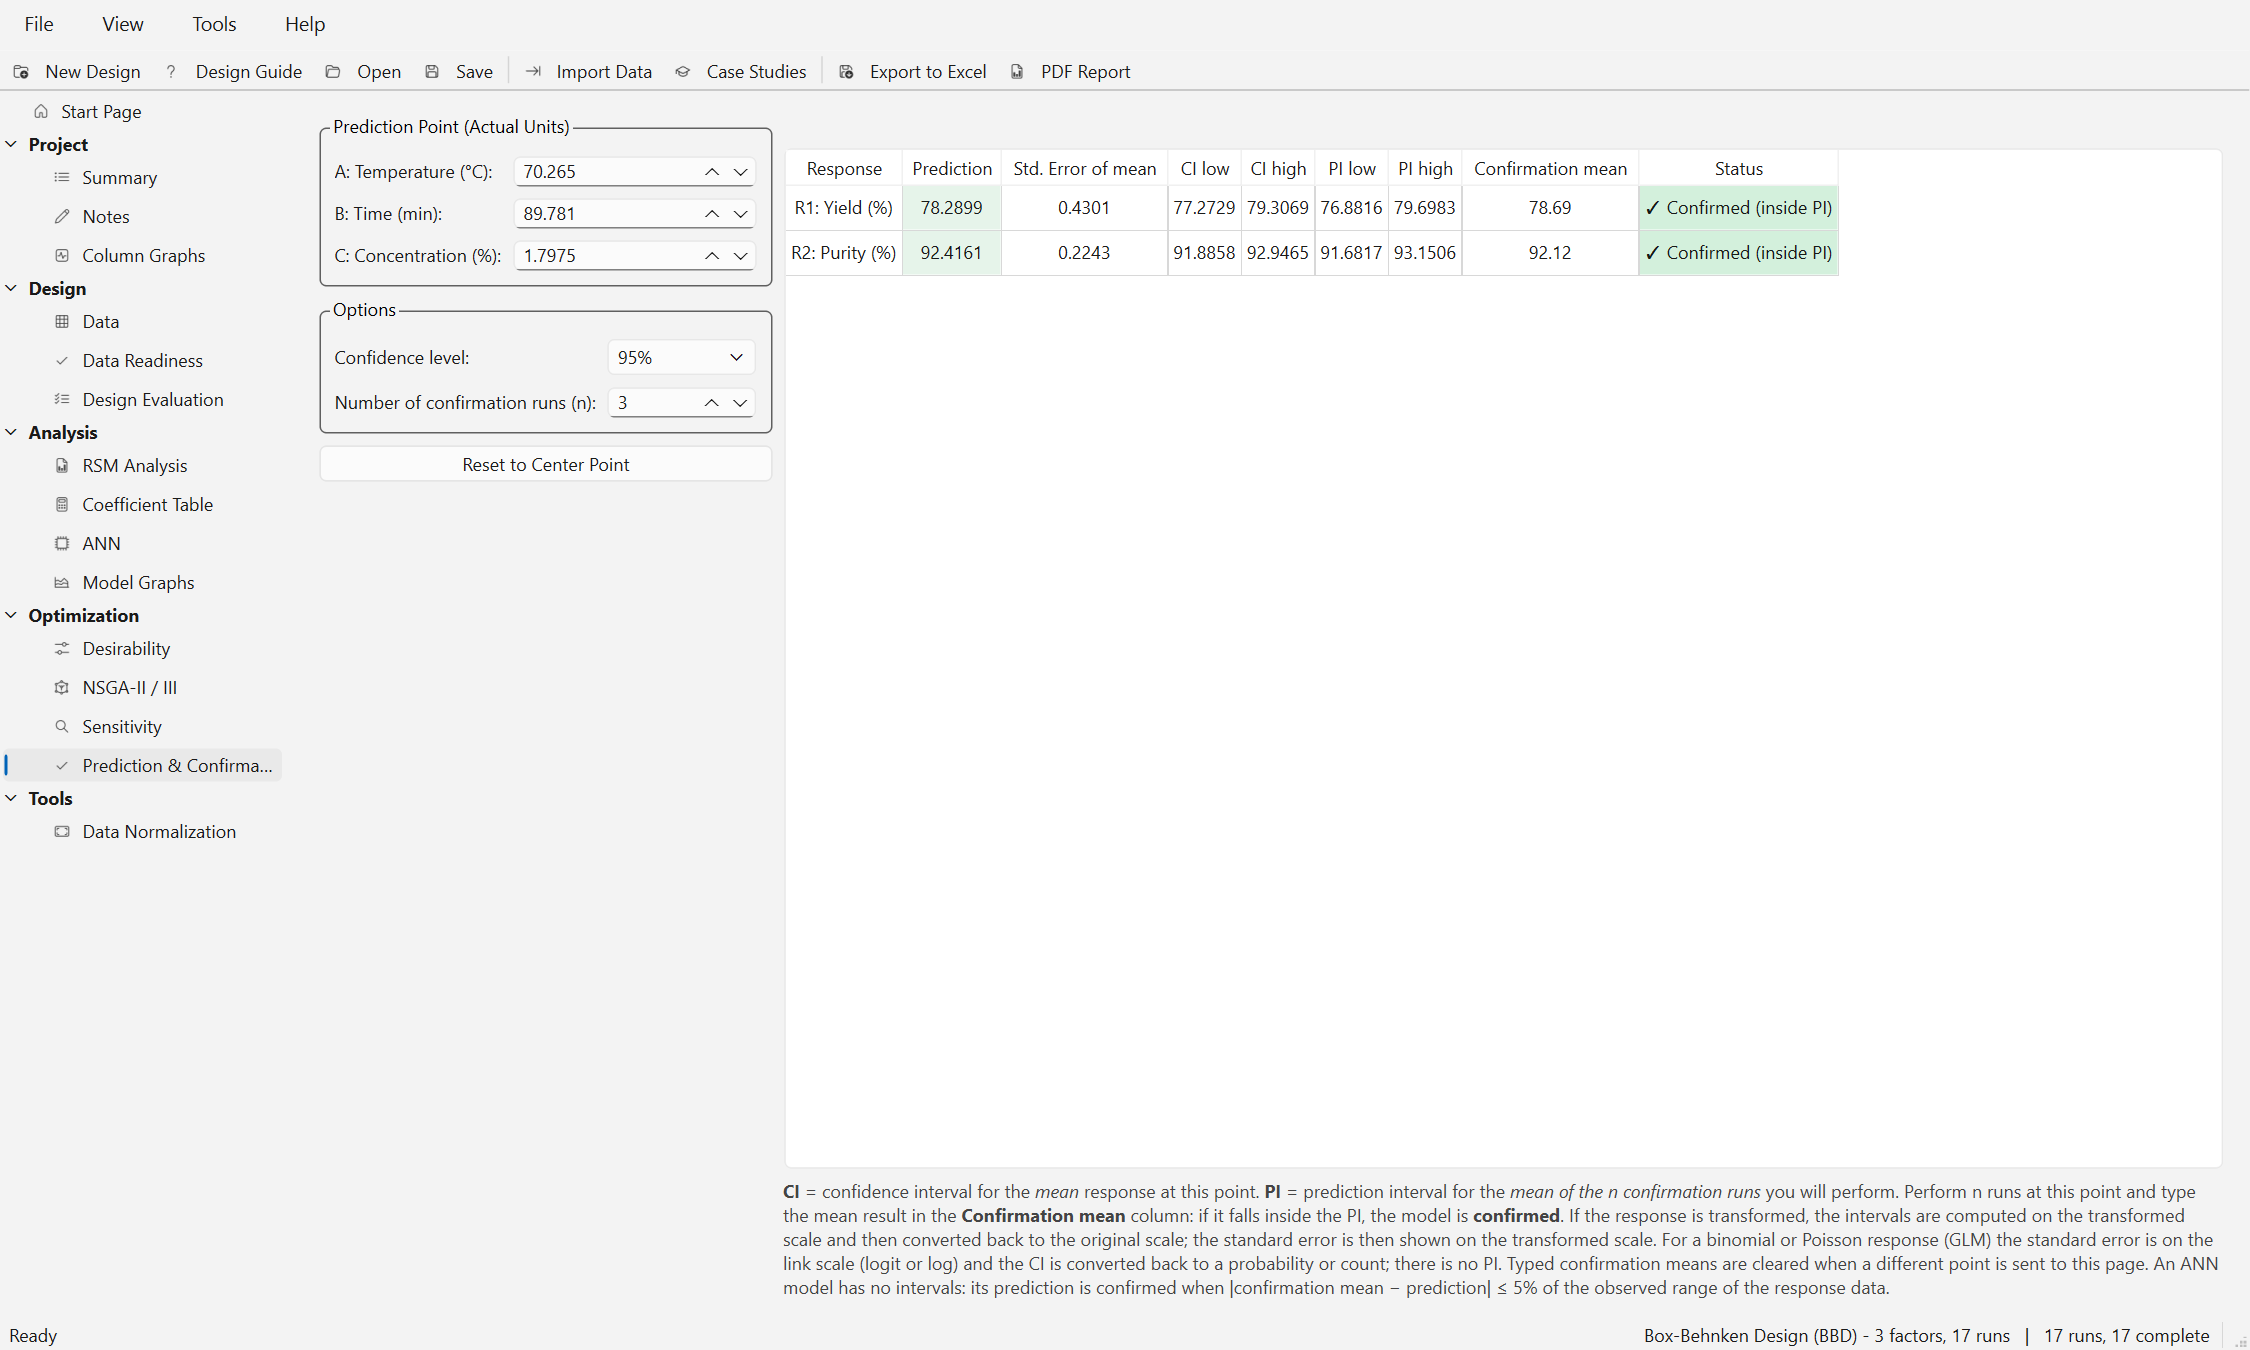
\includegraphics[width=\linewidth]{prediction.png}
\caption{\ui{Prediction \& Confirmation} for the best desirability solution, 95~\%, $n=3$. The confirmation means are
example values.}
\label{fig:ch11-prediction}
\end{figure}

\textbf{Confirmation plan.} Because check~D failed, the plan contains two settings:
\begin{enumerate}
  \item Three runs at the chosen optimum (70.3~°C, 89.8~min, 1.80~\%). Accept the RSM model if both means fall inside
        the PIs above.
  \item One to three runs at the ANN TOPSIS point (65.3~°C, 90.0~min, 3.00~\%). Enter this point on the prediction
        page: the RSM predicts Yield 73.97 with a PI (3 runs) of 72.1--75.8, whereas the ANN predicts 83.5. A measured
        Yield near 74 confirms the RSM and refutes the ANN's promise; a Yield near 83 would mean the RSM misses a
        better region and the design should be extended toward high Concentration.
\end{enumerate}
The \ui{Data Readiness} page also proposes confirmation runs around the optimum (\ui{Add Suggested Runs to Data
Sheet}). After the runs, enter the results on the \ui{Data} page, refit and repeat the checks.

% ======================================================================================================
\section{Part B: dye adsorption, when an ANN is justified}
\label{sec:ch11-dye}
Open \ui{Dye Adsorption (ANN, 40 runs)} from \menupath{File $\rightarrow$ Case Studies\dots}. The data are 40
historical runs with four factors (pH 2--10, adsorbent dose 0.5--4~g/L, contact time 10--120~min, initial concentration
20--200~mg/L) and the response Removal Efficiency (\%).

\subsection{Readiness and RSM}
\ui{Data Readiness} rates the data \ui{Fair - some things need fixing} (modeling 82, optimization 77): there are no
replicates (pure error df 0, \ui{Problem}), so the noise level and the lack of fit cannot be assessed. The quadratic RSM
model (15 parameters) fits with $R^2=0.877$ but predicts new data poorly (predicted $R^2=0.562$): a sign that the
response is more nonlinear than a quadratic surface.

\subsection{Data adequacy}
On \ui{ANN} the \ui{Data Adequacy} verdict is \ui{Adequate with caveats}: 40 runs (\ui{Good}), training rows per
weight 2.62 for a 4-2-1 reference network (\ui{Caution}), factor correlation at most 0.25 (\ui{Good}), skewed response
(skewness 0.85, max/min 21.4, \ui{Caution}), and no replicates for the signal-to-noise ratio (\ui{Info}). For the
skewed response the page points out that a ln transform on the \ui{RSM Analysis} page would change only the RSM model:
the ANN is trained on the response in its original units.

\subsection{Check B: learning curve}
Click \ui{Learning Curve (Enough Data?)} with the default network entry ``5'' (one hidden layer with 5 neurons)
(Figure~\ref{fig:ch11-lc}). The ANN is trained on 30 to 100~\% of the training data (10 to 32 runs) and tested on
8 runs never used for training, repeated 10 times. The median test $R^2$ rises from about 0 at 10 runs to 0.898 at 26
and 0.876 at 32 runs; the RSM reaches only 0.429 on the same test runs. The page concludes \ui{More data would still
help} and estimates about 100 runs in total (range 95 to 111), but adds that this estimate is unreliable because the
fitted exponent lies at the edge of its search range. Read check~B here as: the ANN already clearly beats the RSM with
40 runs, and more runs would still improve it; the exact number of runs is uncertain.

\begin{figure}[htbp]
\centering
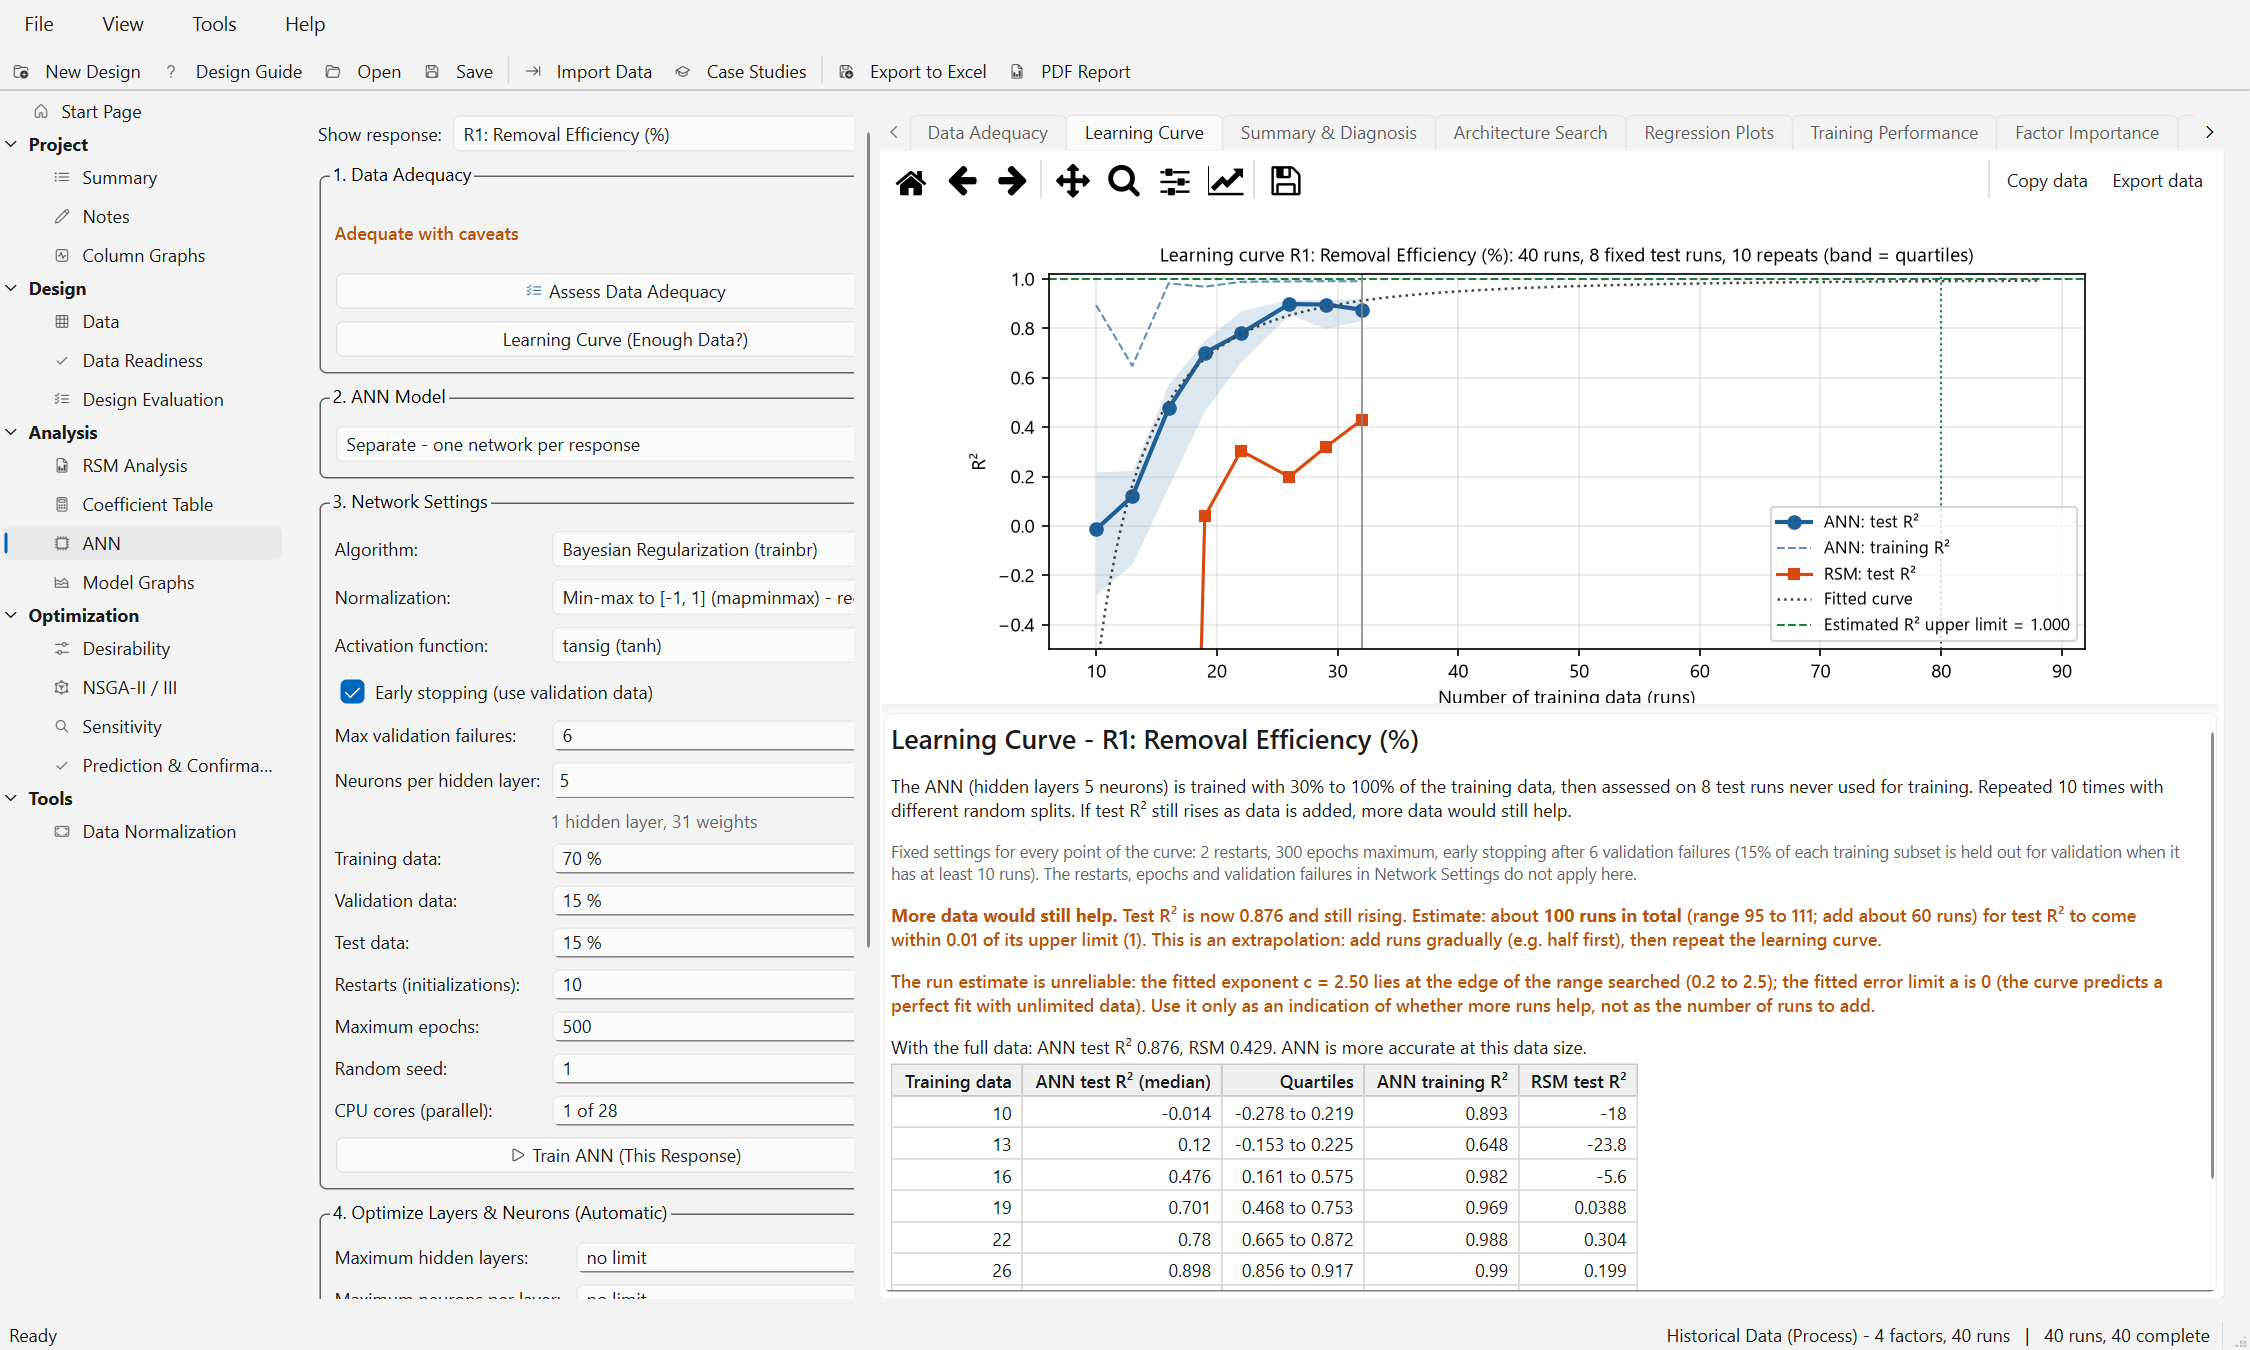
\includegraphics[width=\linewidth]{ann_learning_curve.png}
\caption{Check B for the dye case: learning curve of the ANN (test $R^2$ against training runs) compared with RSM.}
\label{fig:ch11-lc}
\end{figure}

\subsection{Check A: architecture search}
Click \ui{Search Architecture (This Response)} with the default search settings (Figure~\ref{fig:ch11-search}). Fifteen
architectures are evaluated with 5-fold cross-validation. The first hidden layer stops growing at 5 neurons, and a
second layer does not improve the test error by 1~\%. The selected network is 4-3-1 (19 weights): cross-validated
training $R^2$ 0.987, test $R^2$ ($Q^2$) 0.938, \ui{Good fit}; the RSM reaches $Q^2=0.376$ on the same folds. Nine
candidates were excluded as overfitting and three as underfitting.

\begin{figure}[htbp]
\centering
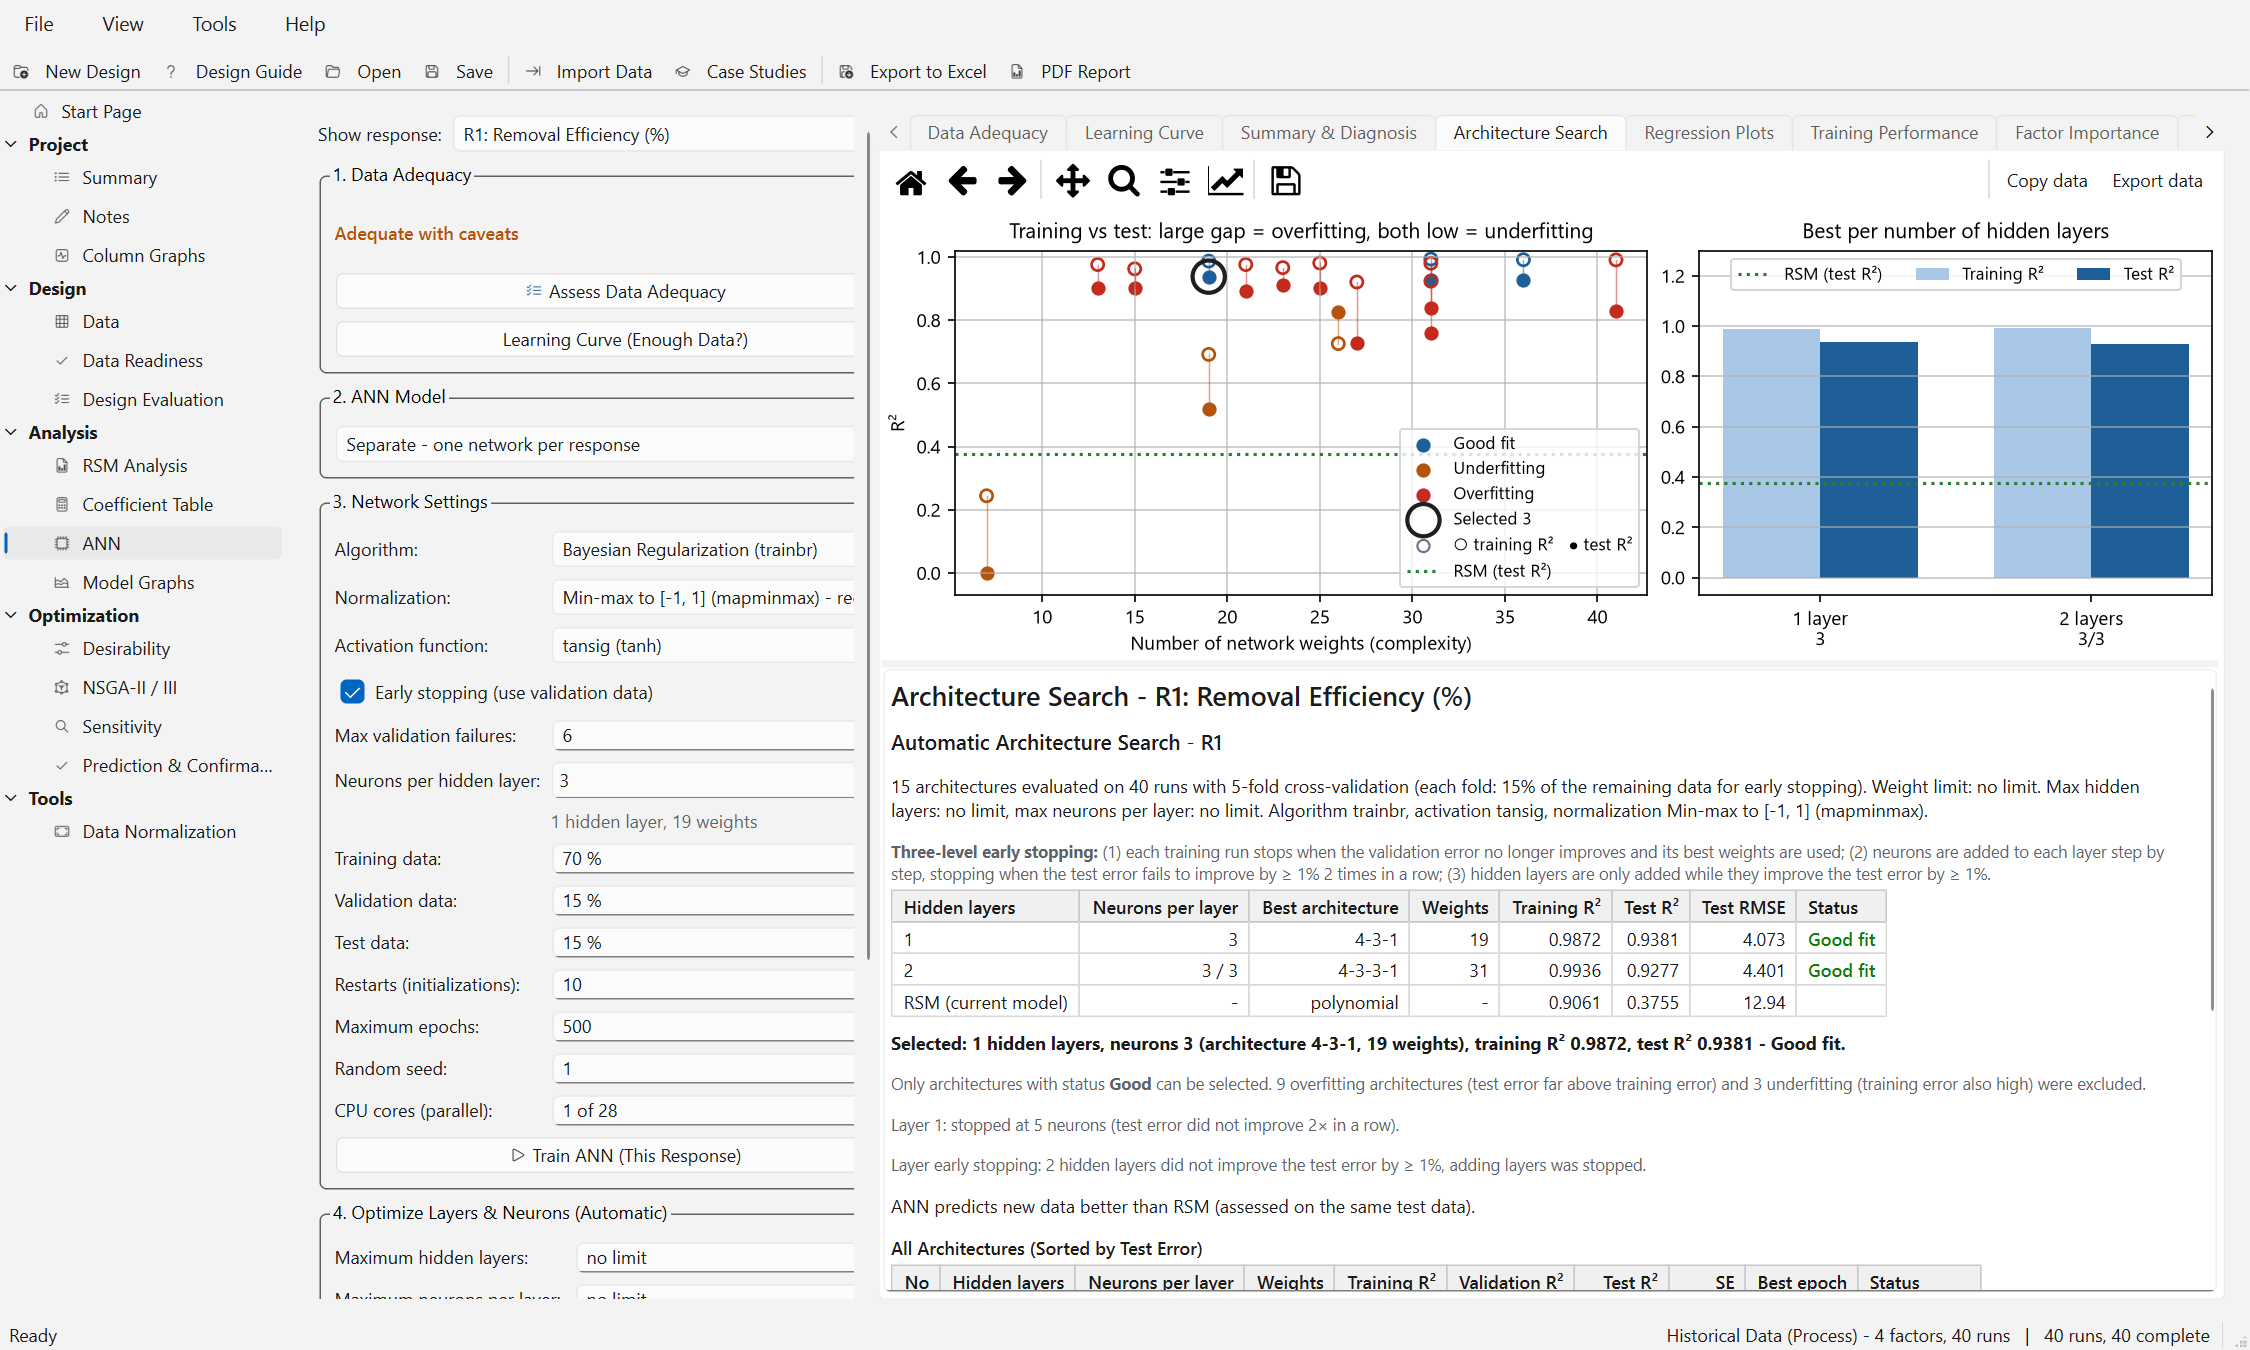
\includegraphics[width=\linewidth]{ann_search.png}
\caption{Check A for the dye case: architecture search with 5-fold cross-validation; selected network 4-3-1.}
\label{fig:ch11-search}
\end{figure}

The final 4-3-1 network is trained on a 28/6/6 split. The \ui{Summary \& Diagnosis} tab reports \ui{Good fit} from the
cross-validation and, for the single final split, \ui{Overfitting} (error on new data 3.6 times the training error,
test $R^2=0.853$). As in Part A, the cross-validated status is the diagnosis to use. The \ui{RSM vs ANN} tab gives
$R^2=0.961$ for the ANN against 0.877 for RSM on all data, and the \ui{Factor Importance (Garson)} tab ranks pH first
(68.2~\%), as expected for an adsorption process with a pH optimum.

\textbf{Conclusion of Part B.} Here an ANN is justified: enough data (40 runs), a clearly nonlinear response that the
quadratic model cannot capture ($Q^2$ 0.94 against 0.38), a network selected by cross-validation, and a learning curve
that confirms the advantage. To use the network for graphs, optimization and prediction, tick \ui{Use this response's
ANN for graphs, optimization, NSGA-II \& prediction}. Keep two limitations in mind: an ANN has no confidence or
prediction intervals, so on the prediction page a confirmation run is judged by the rule $|\bar y-\hat y|\le5$~\% of the
response data range; and the data have no replicates, so the noise level is unknown. Adding a few replicated runs and
the runs suggested by \ui{Data Readiness} would strengthen the model. Multi-objective optimization and check~D need at
least two responses and are therefore not part of this case.

% ======================================================================================================
\section{Export the data and the report}
\label{sec:ch11-export}
Everything shown in this chapter can be exported for a paper or a lab report:
\begin{itemize}
  \item every plot: \ui{Copy data} and \ui{Export data\dots} on the plot toolbar (right-click: \ui{Copy plot data},
        \ui{Export plot data\dots}); the data behind each panel are written to the clipboard, an Excel workbook (one
        sheet per series) or a CSV file, so the figure can be redrawn in another program;
  \item every result table: right-click, \ui{Export table\dots} (Excel or CSV) or \ui{Copy entire table (for Excel)};
  \item every report panel (ANOVA, check reports, sensitivity tables): right-click, \ui{Export all tables\dots};
  \item the Pareto front with settings and convergence history: \ui{Export Pareto to Excel\dots} on the NSGA page;
  \item the whole project: \menupath{File $\rightarrow$ Export to Excel\dots} and \menupath{File $\rightarrow$ PDF
        Report\dots}.
\end{itemize}
The \ui{Summary} page (Figure~\ref{fig:ch11-summary}) collects the state of the project: factor and response tables
(Yield and Purity both quadratic, \ui{Used RSM}), ``2 ANN models, desirability optimization results (5 solutions),
NSGA-II results (99 Pareto solutions)'' and the notes. Save the project (\menupath{File $\rightarrow$ Save}); the models,
optimization results, comparisons and search results are stored in the \texttt{.doe} file.

\begin{figure}[htbp]
\centering
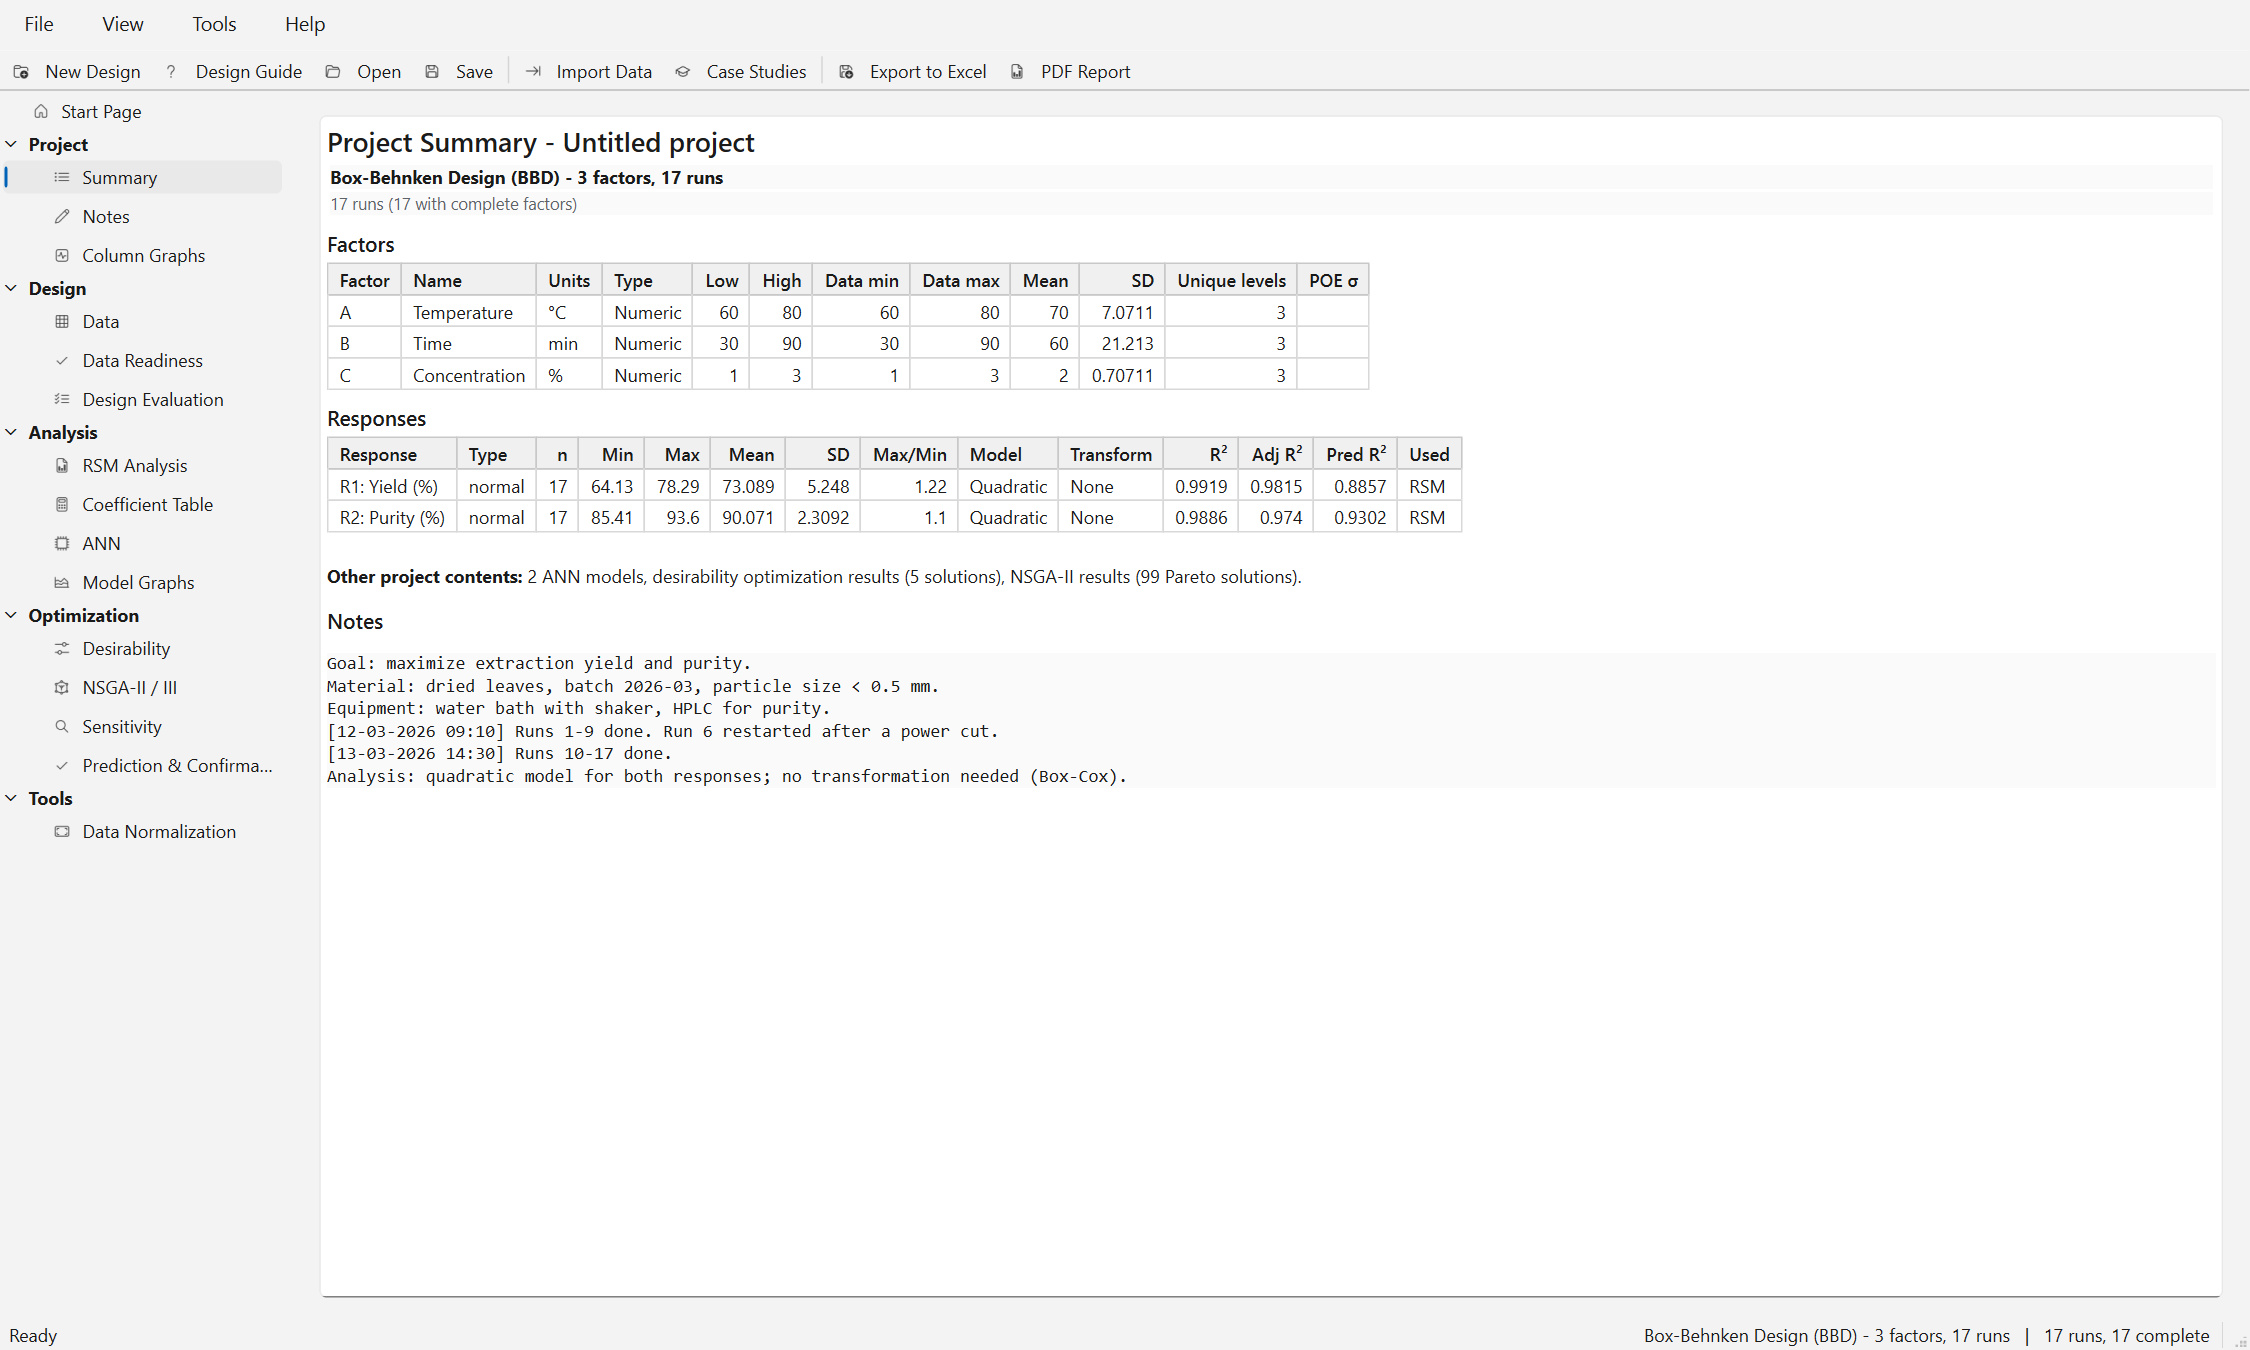
\includegraphics[width=\linewidth]{summary.png}
\caption{\ui{Summary} page of the BBD project at the end of the worked example.}
\label{fig:ch11-summary}
\end{figure}

% ======================================================================================================
\section{Checklist for reporting the study (Part A)}
\label{sec:ch11-checklist}
\begin{table}[htbp]
\centering
\small
\caption{What to report, with the values of the BBD example.}
\label{tab:ch11-checklist}
\begin{tabularx}{\linewidth}{@{}>{\raggedright\arraybackslash}p{2.6cm} >{\raggedright\arraybackslash}X@{}}
\toprule
Item & BBD extraction example \\
\midrule
Design and data & Box-Behnken, 3 factors, 17 runs, 5 center points; readiness \ui{Ready} (94/96 and 100/97). \\
Models & Quadratic RSM; Yield $R^2$ 0.992, predicted $R^2$ 0.886, lack of fit $p=0.030$ (pure error 4 df); Purity $R^2$
0.989, predicted $R^2$ 0.930. \\
Check A & ANN 3-4-1 and 3-5-1 selected by 5-fold CV, $Q^2$ 0.624 and 0.774 (RSM on the same folds 0.598 and 0.818). \\
Check B & ``Too little data to assess''; RSM more accurate at 17 runs. \\
Desirability & Limits 75--78.29 and 89--93.6, importance equal, linear shape; $D=0.862$ at 70.3~°C, 89.8~min,
1.80~\%. \\
NSGA & NSGA-II, population 100, seed 1, automatic stop at generation 78, 99 solutions; TOPSIS 71.5~°C, 88.2~min,
1.88~\%. \\
Check C & Converged (gain $-0.029$~\% $<$ 0.10~\%); population sufficient (seed spread 0.02~\%, 2$\times$ population
+0.35~\%). \\
Check D & Failed: $\Delta=22.4$~\% (Yield), $dx=56$~\%; RSM retained, confirmation at both TOPSIS points. \\
Sensitivity & Sobol $S_T$: Temperature 0.60 / 0.71, Time 0.36 / 0.17, Concentration 0.08 / 0.15 (Yield / Purity). \\
Confirmation & PI (95~\%, $n=3$): Yield 76.9--79.7, Purity 91.7--93.2 at the optimum; Yield 72.1--75.8 at the ANN TOPSIS
point. \\
\bottomrule
\end{tabularx}
\end{table}

% ======================================================================================================
\section{Part C: multi-objective optimization of a polygeneration plant}
\label{sec:ch11-polygen}
Part C follows a complete multi-objective study. The case \ui{Polygeneration Plant (3 Objectives)} contains 80 runs of
an illustrative thermodynamic and thermoeconomic model of a plant that uses geothermal heat to produce power (organic
Rankine cycle), cooling (absorption chiller) and fresh water (reverse osmosis). The runs are simulated with a Latin
hypercube and a small random noise; they are not measurements of a real plant, but they behave the way such a study
does in practice: a plant model is evaluated at space-filling points, a surrogate model is fitted, and the surrogate
is optimized. The five decision variables and the three objectives are:
\begin{itemize}
  \item A: Geothermal Temperature 160--220~°C; B: Turbine Inlet Pressure 1000--2000~kPa; C: Pinch Point 5--15~°C;
        D: RO Recovery Ratio 0.35--0.75; E: Reinjection Temperature 50--90~°C;
  \item Exergy Efficiency (\%, maximize), Product Cost (USD/GJ, minimize), Environmental Impact (mPts/h, minimize).
\end{itemize}
The goals are preset by the case. The settings are the defaults unless stated (ANN seed 1, NSGA seed 1, one CPU core).

\subsection{Readiness}
\ui{Data Readiness} (reference model Quadratic, 21 parameters) rates all three responses \ui{Ready}: modeling scores 92,
92 and 92, optimization scores 91, 94 and 91. The structure is sound (80 complete runs, residual df 59, 79 to 80
distinct levels per factor, maximum VIF 1.63, largest gap in the factor space 0.29), and there are no outliers. Two
items need attention: there are no replicates (pure error df 0, \ui{Problem}), so the noise level and the lack of fit
cannot be assessed, and six runs have high leverage. Without replicates the honest statement is that the surrogate
reproduces the plant model, not that the noise is known; for a simulated data set this is acceptable.

The readiness report also locates the model optimum of each response, and these already show the conflict: the
highest Exergy Efficiency lies at A~=~219.6~°C, B~=~1901~kPa, C~=~5.1~°C, D~=~0.352, E~=~50.8~°C, the lowest Product
Cost at A~=~218.8~°C, E~=~52.0~°C, but the lowest Environmental Impact at A~=~160.9~°C, B~=~1192~kPa, E~=~83.3~°C, at
the other end of the temperature range.

\subsection{Response surface models}
On \ui{RSM Analysis}, \ui{Fit Summary} suggests the quadratic model for all three responses (Exergy Efficiency:
adjusted $R^2$ 0.9947, predicted $R^2$ 0.9923; Product Cost: 0.9767 and 0.9672; Environmental Impact: 0.9924 and
0.9901). The cubic model has a lower predicted $R^2$ for every response (0.9651, 0.9202 and 0.9453), a sign of
overfitting. All five main effects are significant for Exergy Efficiency (model $F=743.5$) and Environmental Impact
($F=516.5$); for Product Cost the linear term of the RO Recovery Ratio is not ($p=0.070$), although its quadratic term
is part of the model. Among the interactions, Geothermal Temperature $\times$ Reinjection Temperature (AE) is significant
for Exergy Efficiency and Geothermal Temperature $\times$ Turbine Inlet Pressure (AB) for Environmental Impact
($p=0.0035$).

\subsection{ANN with checks A and B}
Even with excellent RSM models, the ANN checks are worth running, because check~D needs the networks. On \ui{ANN} the
\ui{Data Adequacy} verdict is \ui{Adequate for ANN modeling} for all three responses. \ui{Optimize All Responses (One
Click)} (check~A) selects:
\begin{itemize}
  \item Exergy Efficiency: 5-3-1 (22 weights), $Q^2=0.9904$; RSM on the same folds 0.9924;
  \item Product Cost: 5-8-4-1 (89 weights), $Q^2=0.9548$; RSM 0.9623;
  \item Environmental Impact: 5-4-1 (29 weights), $Q^2=0.9875$; RSM 0.9892.
\end{itemize}
All three networks are \ui{Good fit}, and each search ends with \ui{RSM predicts new data as well as or better than
ANN (assessed on the same test data)}. The learning curves (check~B) agree: with the full data the ANN reaches a test
$R^2$ of 0.984, 0.964 and 0.984 against 0.991, 0.970 and 0.989 for the RSM (\ui{RSM is more accurate at this data
size}). For Exergy Efficiency and Product Cost the curve is still rising (\ui{More data would still help}), with a run
estimate that the page itself marks as unreliable; for Environmental Impact \ui{The data is sufficient}.

\textbf{Decision.} The RSM models stay selected. The response is smooth, the quadratic surface captures it, and the
networks bring no gain. This is the opposite of the turning case of Chapter~\ref{chap:8}, and it is a normal outcome:
an ANN is justified only when it predicts new data better.

\subsection{NSGA-III and check C}
On \ui{NSGA-II / III} the three goals are already set. The first run with all defaults (population 100, max
generations 300) chooses NSGA-III with 91 reference points and runs all 300 generations. Check~C is not passed: the
quick assessment reads \ui{Not enough generations yet: the mean hypervolume of the last 20 generations is still rising
-0.203\% and the ideal point shifted 1.83\%.} (the hypervolume itself no longer rises; it is the ideal point, the best
value of each objective, that still moves by more than 1~\%), and it adds that all 100 individuals are on the first
front. Raising \ui{Max generations:} to 600 does not help: after 600 generations the ideal point still shifts by
2.19~\%. \ui{Check Population Size} shows where the problem lies: two other seeds change the hypervolume by $+0.27$~\%
and $+1.07$~\%, and a population of 200 adds 3.24~\% and converges after 145 generations, whereas all three runs with
100 individuals use the full 300 generations. The verdict is \ui{Generations: not sufficient, increase the maximum
generations.} and \ui{Population: not sufficient (the result changes by 1.1\% when the seed is changed; a 2x population
increases the hypervolume by 3.2\%). Increase the population, for example to 200, then check again.} A population of
100 is too small to hold the ends of this three-objective front with five decision variables, so the extremes of the
front keep moving.

With \ui{Population:} 200 (190 reference points) the run stops automatically at generation 145 with 197 Pareto
solutions: \ui{Enough generations: the mean hypervolume of the last 20 generations changed by only +0.045\% compared
with the previous 20 generations (limit 0.19\%) and the ideal point shifted 0.16\% (limit 1\%).} The result line is
\ui{NSGA-III: 197 Pareto solutions, automatic stop at generation 145. Best compromise (TOPSIS): Geothermal Temperature =
218.51, Turbine Inlet Pressure = 1401.3, Pinch Point = 10.665, RO Recovery Ratio = 0.74987, Reinjection Temperature =
50.589 $\rightarrow$ Exergy Efficiency = 20.132, Product Cost = 18.194, Environmental Impact = 3.9337}.

\ui{Check Population Size} for this run (Table~\ref{tab:ch11-poly-popcheck}) reports \ui{Generations: sufficient (the
hypervolume has flattened).} but \ui{Population: not sufficient (the result changes by 1.2\% when the seed is changed; a
2x population increases the hypervolume by 1.4\%). Increase the population, for example to 400, then check again.} Both
values are only slightly above the 1~\% limit. A run with population 400 (378 reference points) stops at generation
115 with 389 solutions, and its own population check is passed: \ui{Population: sufficient. Another seed changes the
hypervolume by only 0.66\% and a 2x population adds only 0.98\%.}

\begin{table}[htbp]
\centering
\small
\caption{\ui{Adequacy Check Results} for the polygeneration case (NSGA-III, RSM models, seed 1) with population 200 and
400.}
\label{tab:ch11-poly-popcheck}
\begin{tabular}{@{}lrrlrrrr@{}}
\toprule
Run & Pop. & Seed & Generations & Solutions & HV & Diff. & TOPSIS shift (\%) \\
\midrule
Current result & 200 & 1 & 145 (converged) & 197 & 58.90\% & +0.00\% & 0.0 \\
Different seed & 200 & 102 & 300 & 196 & 58.79\% & $-0.19$\% & 13.5 \\
Different seed 2 & 200 & 203 & 120 (converged) & 190 & 58.21\% & $-1.17$\% & 5.5 \\
Population 2x & 400 & 1 & 115 (converged) & 389 & 59.73\% & +1.40\% & 13.7 \\
\midrule
Current result & 400 & 1 & 115 (converged) & 389 & 58.71\% & +0.00\% & 0.0 \\
Different seed & 400 & 102 & 130 (converged) & 392 & 58.33\% & $-0.65$\% & 7.7 \\
Different seed 2 & 400 & 203 & 110 (converged) & 391 & 58.44\% & $-0.46$\% & 5.4 \\
Population 2x & 800 & 1 & 100 (converged) & 781 & 59.29\% & +0.99\% & 3.7 \\
\bottomrule
\end{tabular}
\end{table}

How much does this matter for the decision? The TOPSIS choice of the population-400 run is 216.04~°C, 1372.4~kPa,
12.031~°C, 0.750, 50.002~°C with Exergy Efficiency 19.59~\%, Product Cost 18.00~USD/GJ and Environmental Impact
3.848~mPts/h. Compared with the population-200 choice, only the Pinch Point moves noticeably (12.0 against 10.7~°C,
13.7~\% of its range), and the objectives change by 0.54 percentage points of efficiency, 0.19~USD/GJ and
0.085~mPts/h, small against the ranges of the front. The front is flat in the Pinch Point direction: a slightly larger
pinch trades a little efficiency for a little cost and impact. The rest of this part uses the population-200 run,
which is the one shown in the screenshots; with population 400 the conclusions are the same. In a report, state the
population that passed check~C (400) and the run used for the figures.

\begin{figure}[htbp]
\centering
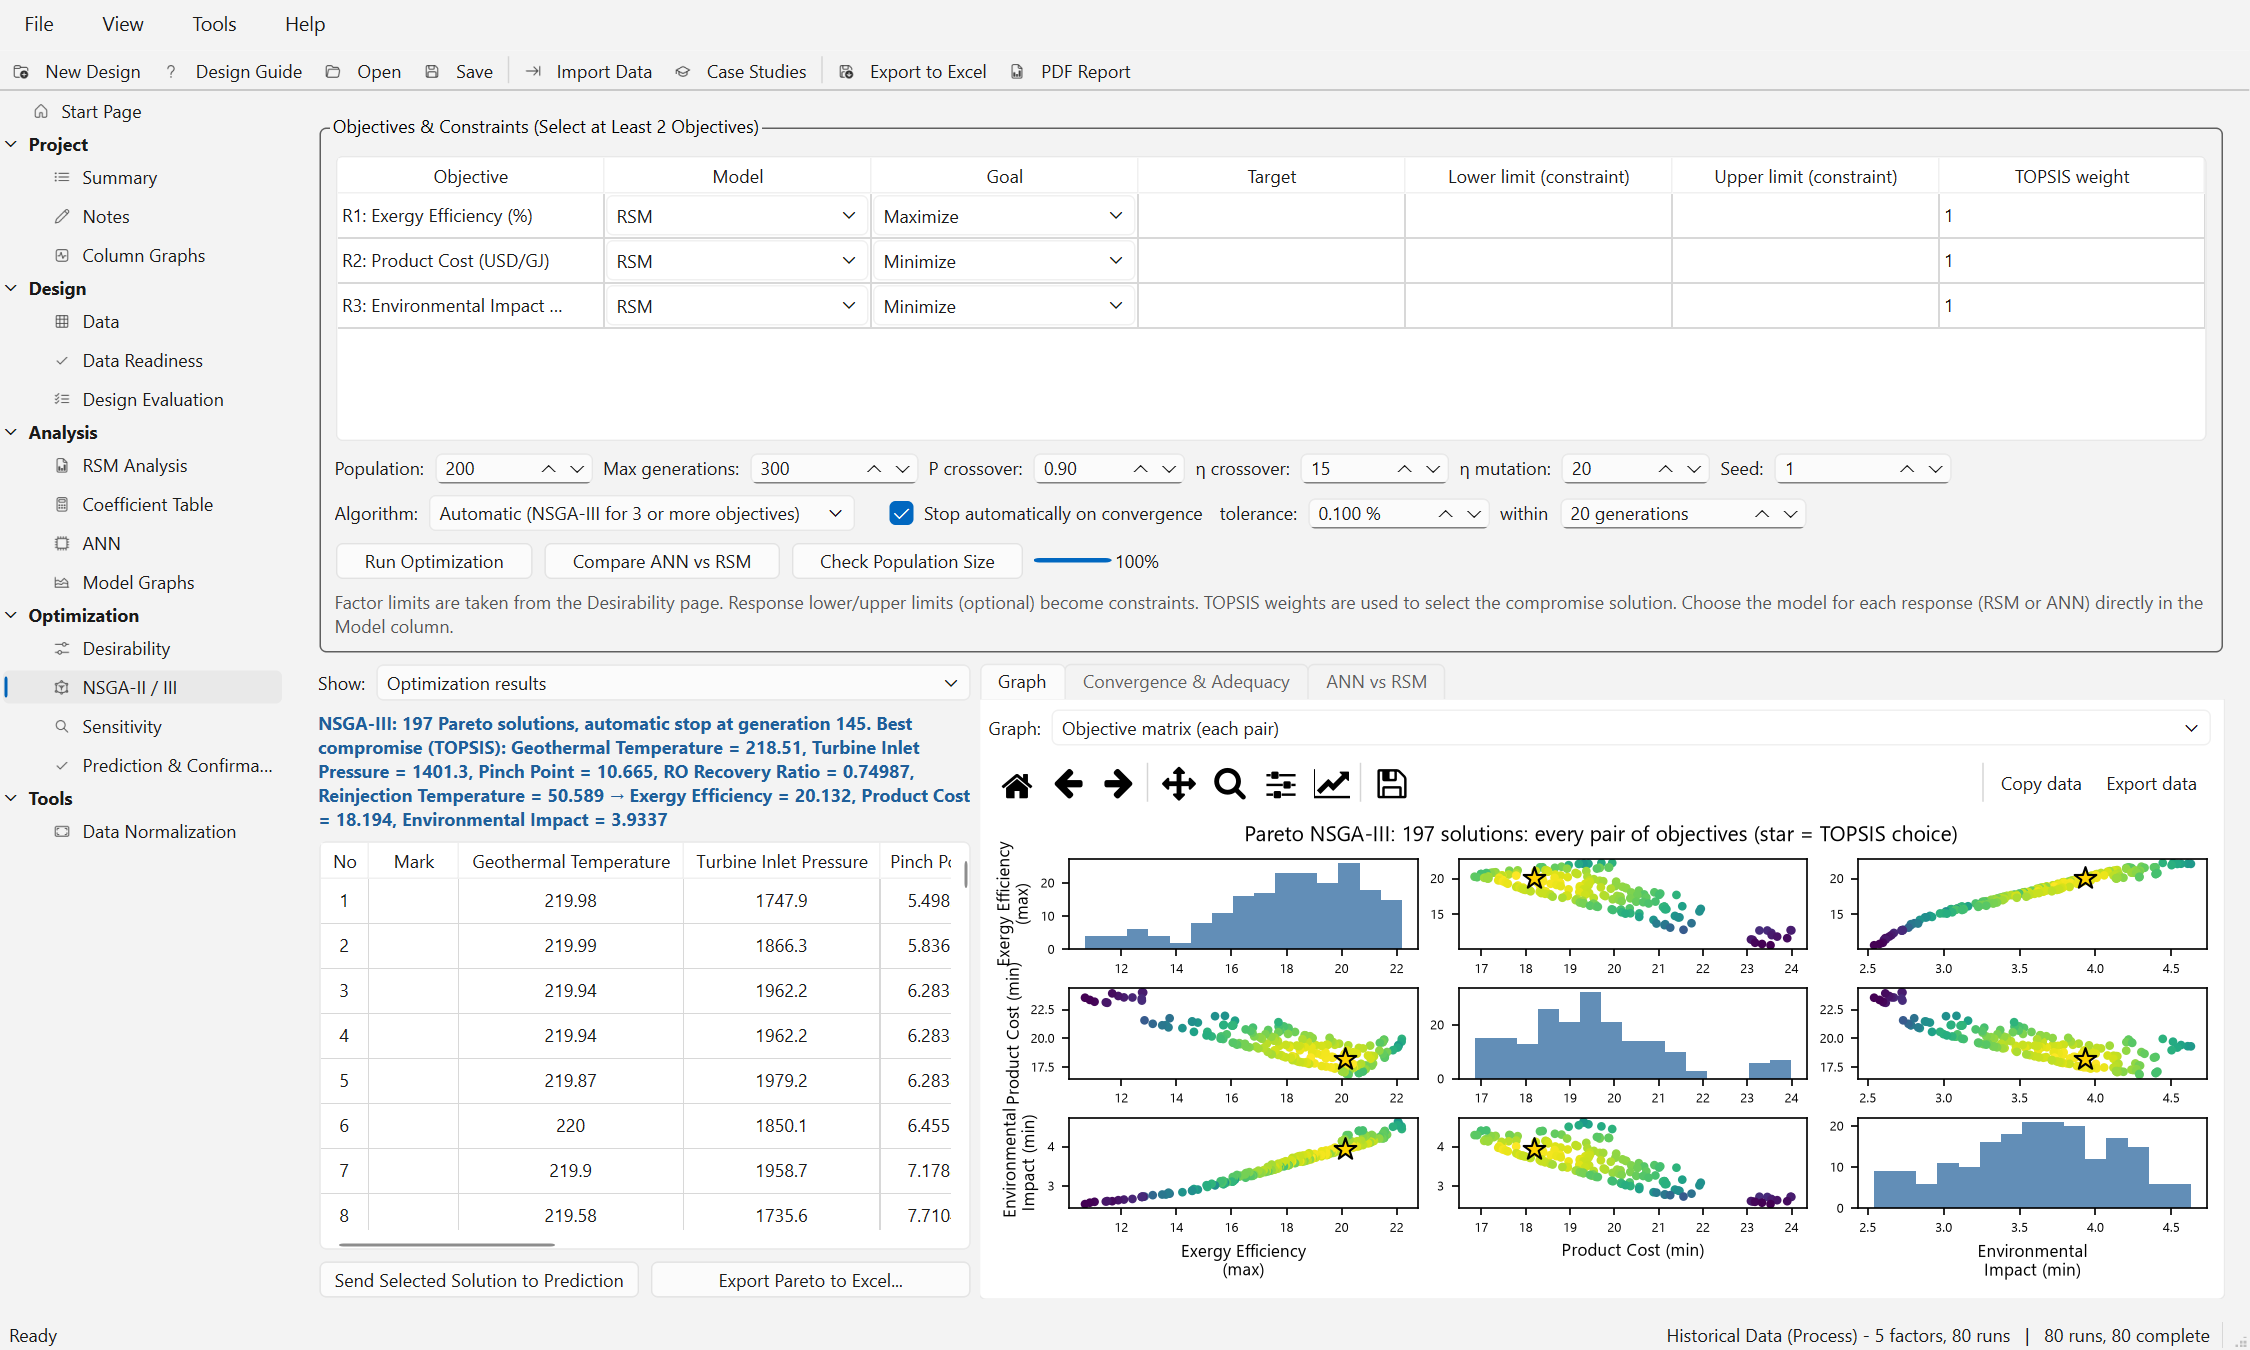
\includegraphics[width=\linewidth]{moo_polygen_front.png}
\caption{NSGA-III front of the polygeneration case (population 200, 197 solutions), \ui{Objective matrix (each pair)}.
Exergy Efficiency and Environmental Impact rise together (conflict), Exergy Efficiency and Product Cost improve
together; the star is the TOPSIS choice.}
\label{fig:ch11-poly-front}
\end{figure}

The objective matrix (Figure~\ref{fig:ch11-poly-front}) shows the shape of the front: Exergy Efficiency ranges from
10.68 to 22.19~\%, Product Cost from 16.85 to 24.00~USD/GJ and Environmental Impact from 2.54 to 4.63~mPts/h.
Efficiency and impact rise together along an almost straight band, while the cost falls as the efficiency rises.

\subsection{Check D: ANN versus RSM}
\ui{Compare ANN vs RSM} with the same settings (population 200, seed 1) gives the green verdict \ui{Both models agree:
predictions on the front differ by only 3.0\% on average and the compromise choices are close together. The
optimization result does not depend on the choice of model.} The details:
\begin{itemize}
  \item fronts of 197 (RSM, 145 generations) and 198 solutions (ANN, 100 generations); hypervolume 58.7~\% and
        58.3~\% by the own model, 57.3~\% and 58.1~\% by the other model;
  \item mean (maximum) prediction difference on the fronts: Exergy Efficiency 1.9~\% (7.2~\%), Product Cost 3.0~\%
        (10.8~\%), Environmental Impact 1.6~\% (5.4~\%) of the data range;
  \item TOPSIS choices: RSM front 218.51~°C, 1401.3~kPa, 10.665~°C, 0.7499, 50.589~°C (Exergy Efficiency 20.132 by RSM
        and 20.151 by ANN, Product Cost 18.194 and 18.047, Environmental Impact 3.9337 and 3.9691); ANN front
        216.24~°C, 1412.6~kPa, 12.063~°C, 0.7499, 50.011~°C (19.738 and 19.793, 17.929 and 17.852, 3.8768 and
        3.9191). The distance is $dx=14.0$~\%, just inside the 15~\% limit, and it comes from the Pinch Point (10.7
        against 12.1~°C): the front is flat in that direction;
  \item accuracy on new data: RSM mean predicted $R^2$ 0.983, ANN mean cross-validation $Q^2$ 0.978.
\end{itemize}
Check~D is passed. Together with checks A and B it says that the result does not depend on the surrogate: two
different model families, fitted to the same 80 runs, lead to the same trade-off and to compromise settings whose
predicted objectives differ by less than 0.4~percentage points of efficiency.

\subsection{Sensitivity and parametric study}
On \ui{Sensitivity} choose \ui{Start from:} \ui{NSGA: TOPSIS choice} and \ui{Model:} \ui{Selected model of each
response}. The results are discussed in Section~\ref{sec:ch09-polygen} of Chapter~\ref{chap:9}
(Figures~\ref{fig:ch09-poly-param}--\ref{fig:ch09-poly-front}); in short:
\begin{itemize}
  \item the Geothermal Temperature sets the trade-off: it has the largest standardized coefficient for all three
        objectives ($+0.727$, $-0.582$, $+0.844$) and the largest Sobol index for efficiency (0.465) and impact
        (0.604), and it changes steadily along the front ($\rho=0.95$ with efficiency);
  \item the Pinch Point is the second lever for the cost (Sobol $S_T=0.365$), the Turbine Inlet Pressure for the
        impact (0.202);
  \item Reinjection Temperature and RO Recovery Ratio stay near one of their bounds on most of the front (about
        50~°C and 0.75): they can be fixed there;
  \item the responses are almost additive (sum of $S_1$ at least 0.996).
\end{itemize}
\ui{Local Sensitivity (Tornado)} with $\pm10$~\% adds the view from the chosen point: the Exergy Efficiency (20.132)
changes most with the Turbine Inlet Pressure (19.764 at 1301~kPa, 20.433 at 1501~kPa) and the Geothermal Temperature
(19.623 at 212.5~°C, 20.258 at 220~°C), and the Product Cost (18.194) most with the Pinch Point (18.492 at 9.66~°C,
17.957 at 11.66~°C). In the plant these are the variables to control most tightly around the chosen setting.

\subsection{Choice of the compromise}
The front offers a continuum of designs, and the choice depends on how much the environmental impact weighs against
efficiency and cost. Two candidates are marked on the page:
\begin{itemize}
  \item TOPSIS (equal weights): 218.51~°C, 1401.3~kPa, 10.665~°C, 0.7499, 50.589~°C with Exergy Efficiency 20.13~\%,
        Product Cost 18.19~USD/GJ and Environmental Impact 3.934~mPts/h;
  \item knee point: 201.34~°C, 1424.3~kPa, 13.618~°C, 0.7475, 50.128~°C with Exergy Efficiency 18.20~\%, Product
        Cost 18.45~USD/GJ and Environmental Impact 3.619~mPts/h.
\end{itemize}
Moving from the TOPSIS choice to the knee lowers the impact by 8~\% (3.934 to 3.619) and costs 1.93 percentage points
of efficiency and 0.26~USD/GJ. Both lie in the interior of the front, away from its ends (efficiency 10.7 and
22.2~\%), where the models are least supported by data. In this example the TOPSIS choice is taken as the design point,
and the knee is kept as the low-impact alternative. Other preferences are expressed with the \ui{TOPSIS weight}
column, or by a response limit, for example an \ui{Upper limit (constraint)} on the Environmental Impact.

\subsection{Confirmation plan}
\ui{Send Selected Solution to Prediction} (without a selection the TOPSIS solution is sent) gives the predictions with
their intervals. Because the runs come from a deterministic plant model, ``confirmation'' here means one new evaluation
of the plant model at the chosen point, so set \ui{Number of confirmation runs (n):} to 1. The 95~\% prediction
intervals for a single run are then:
\begin{itemize}
  \item TOPSIS point: Exergy Efficiency 19.74--20.53~\%, Product Cost 17.61--18.78~USD/GJ, Environmental Impact
        3.848--4.019~mPts/h;
  \item knee point: 17.79--18.62~\%, 17.83--19.08~USD/GJ, 3.528--3.710~mPts/h.
\end{itemize}
With the default $n=3$ (for repeated measurements on a real plant or pilot unit) the intervals at the TOPSIS point are
19.82--20.44~\%, 17.73--18.66~USD/GJ and 3.866--4.001~mPts/h. Evaluate the plant model at both points; if the values
fall inside the intervals, the surrogate is confirmed where it matters. Because the data have no replicates, the
residual variance behind these intervals contains the small lack of fit of the quadratic models as well as the noise,
so they are, if anything, slightly conservative. If a value falls outside, add the evaluated point to the data, refit
and repeat the optimization.

\subsection{Export of the data}
For a report or paper the following exports cover the study:
\begin{itemize}
  \item \ui{Export Pareto to Excel\dots} on the NSGA page: the 197 solutions with factor values, all responses and the
        TOPSIS score (sheet \texttt{Pareto}), the settings and the stop reason (\texttt{Settings}), the convergence
        history (\texttt{Convergence}) and, after check~D, the sheets \texttt{RSM Front}, \texttt{ANN Front} and
        \texttt{ANN vs RSM};
  \item the reports of check~C (\ui{Convergence \& Adequacy}) and check~D (\ui{ANN vs RSM}) with \ui{Export all
        tables\dots};
  \item the significance table, the Sobol tables, the tornado tables and the Spearman tables of the
        \ui{Sensitivity} page with \ui{Export all tables\dots}, and the data behind every graph (for example the
        parametric curves) with \ui{Export data\dots};
  \item the ANOVA tables and fit summaries of the three RSM models, and the architecture search tables of the ANN
        page;
  \item the whole project with \menupath{File $\rightarrow$ Export to Excel\dots} and \menupath{File $\rightarrow$
        PDF Report\dots}.
\end{itemize}

% ======================================================================================================
\section{Part C, mixture variant: concrete mix paste}
\label{sec:ch11-concrete}
The case \ui{Concrete Mix Paste (Mixture, 3 Objectives)} shows the same workflow for a constrained mixture: cement
(45--75~\%), fly ash (0--30~\%) and water (20--35~\%) of the paste, with the water/binder ratio limited to 0.35--0.60
by two linear constraints, 14 runs of a D-optimal design and quadratic Scheff\'e models (predicted $R^2$ 0.993, 0.984
and 0.997). Compressive Strength is maximized, Material Cost and CO2 Emission are minimized. Two things differ from a
process study. First, the factors are not independent: NSGA-III works on the simplex and repairs every new blend so
that the components sum to 100~\%, and the constraints are handled as violations
(Section~\ref{sec:ch08-nsga} of Chapter~\ref{chap:8}). Second, the Sobol indices are not available for a pure mixture,
because mixture components cannot vary one at a time; the trade-off is read from the front and the ternary graphs.

With the defaults NSGA-III stops at generation 120 with 92 solutions (Figure~\ref{fig:ch11-concrete-front}). The front
runs from 32.5 to 52.7~MPa, 84.9 to 99.8~USD/t and 425 to 661~kg/t of CO2. Up to 45.9~MPa the cement content stays at
its minimum of 45--45.6~\%, and the strength is gained by replacing water with fly ash (fly ash 20 to 29~\%, water 35 to
26~\%); the CO2 emission stays between 425 and 432~kg/t while the cost rises. Beyond that point more cement is the only
way to more strength, and the CO2 jumps to 478~kg/t at 46.2~MPa and above 600~kg/t from about 48.5~MPa. The TOPSIS
choice sits exactly at this step:
cement 45.0~\%, fly ash 29.0~\%, water 26.0~\% with 45.89~MPa, 94.27~USD/t and 428.4~kg/t. The desirability
optimization with the preset goals (limits = data range) finds a neighbouring blend, cement 45~\%, fly ash 27.8~\%,
water 27.2~\% ($D=0.626$), shown in the ternary desirability contour (Figure~\ref{fig:ch11-concrete-desir}).

\begin{figure}[htbp]
\centering
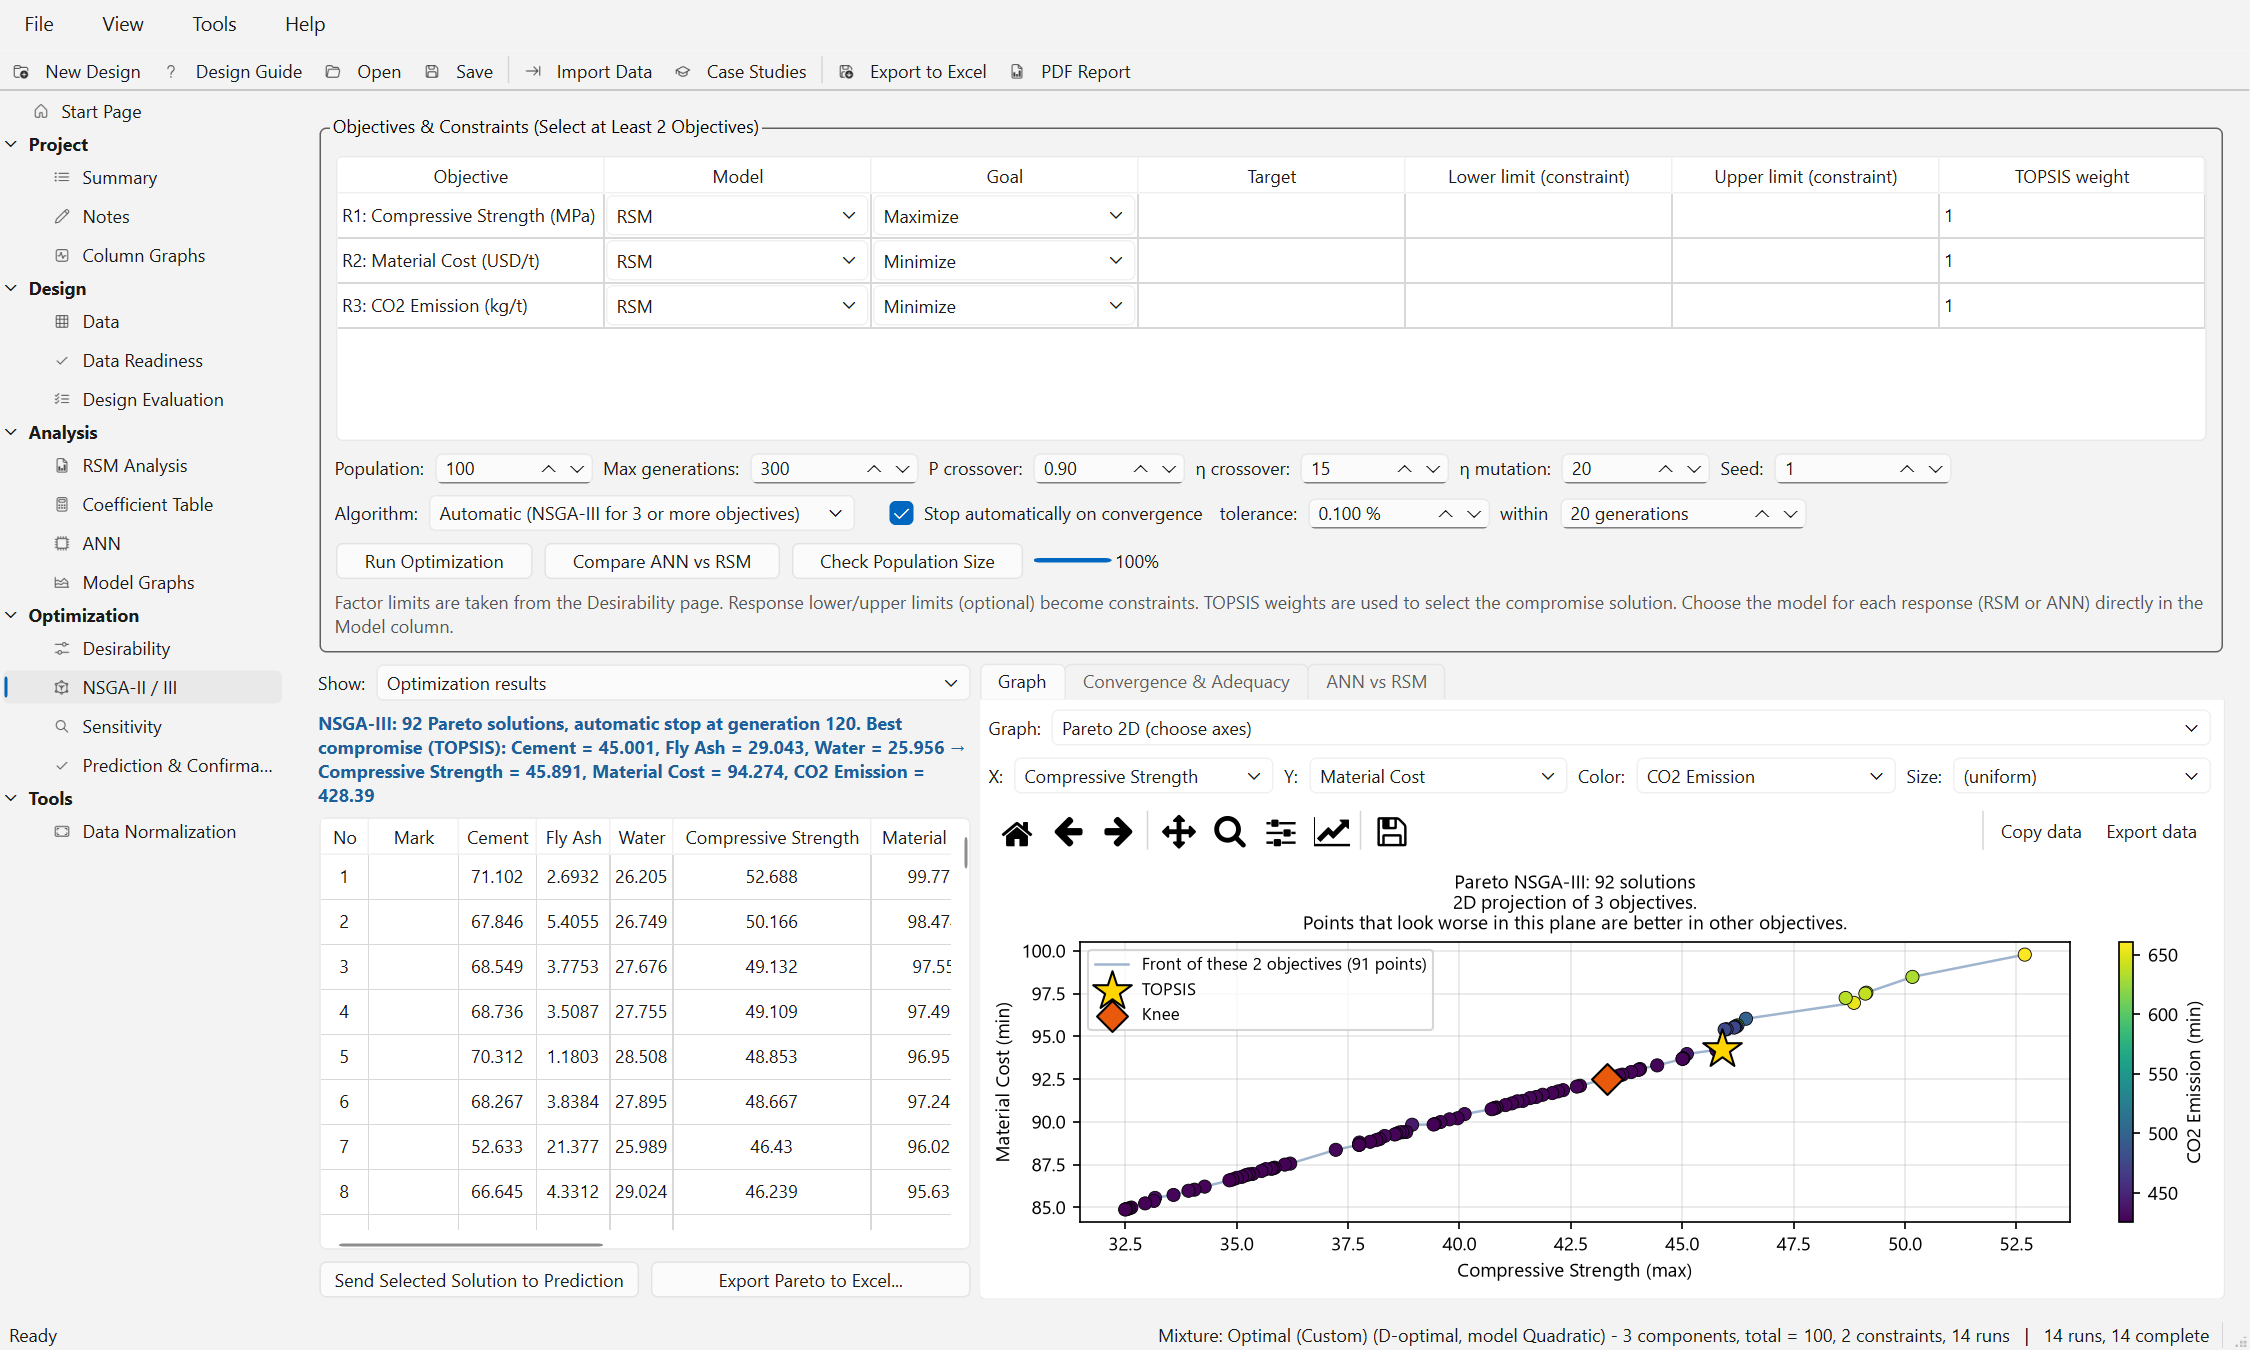
\includegraphics[width=\linewidth]{moo_concrete_front.png}
\caption{NSGA-III front of the concrete mix paste, \ui{Pareto 2D (choose axes)}: Compressive Strength against Material
Cost, colored by CO2 Emission. Beyond about 46~MPa the emission jumps (yellow points).}
\label{fig:ch11-concrete-front}
\end{figure}

\begin{figure}[htbp]
\centering
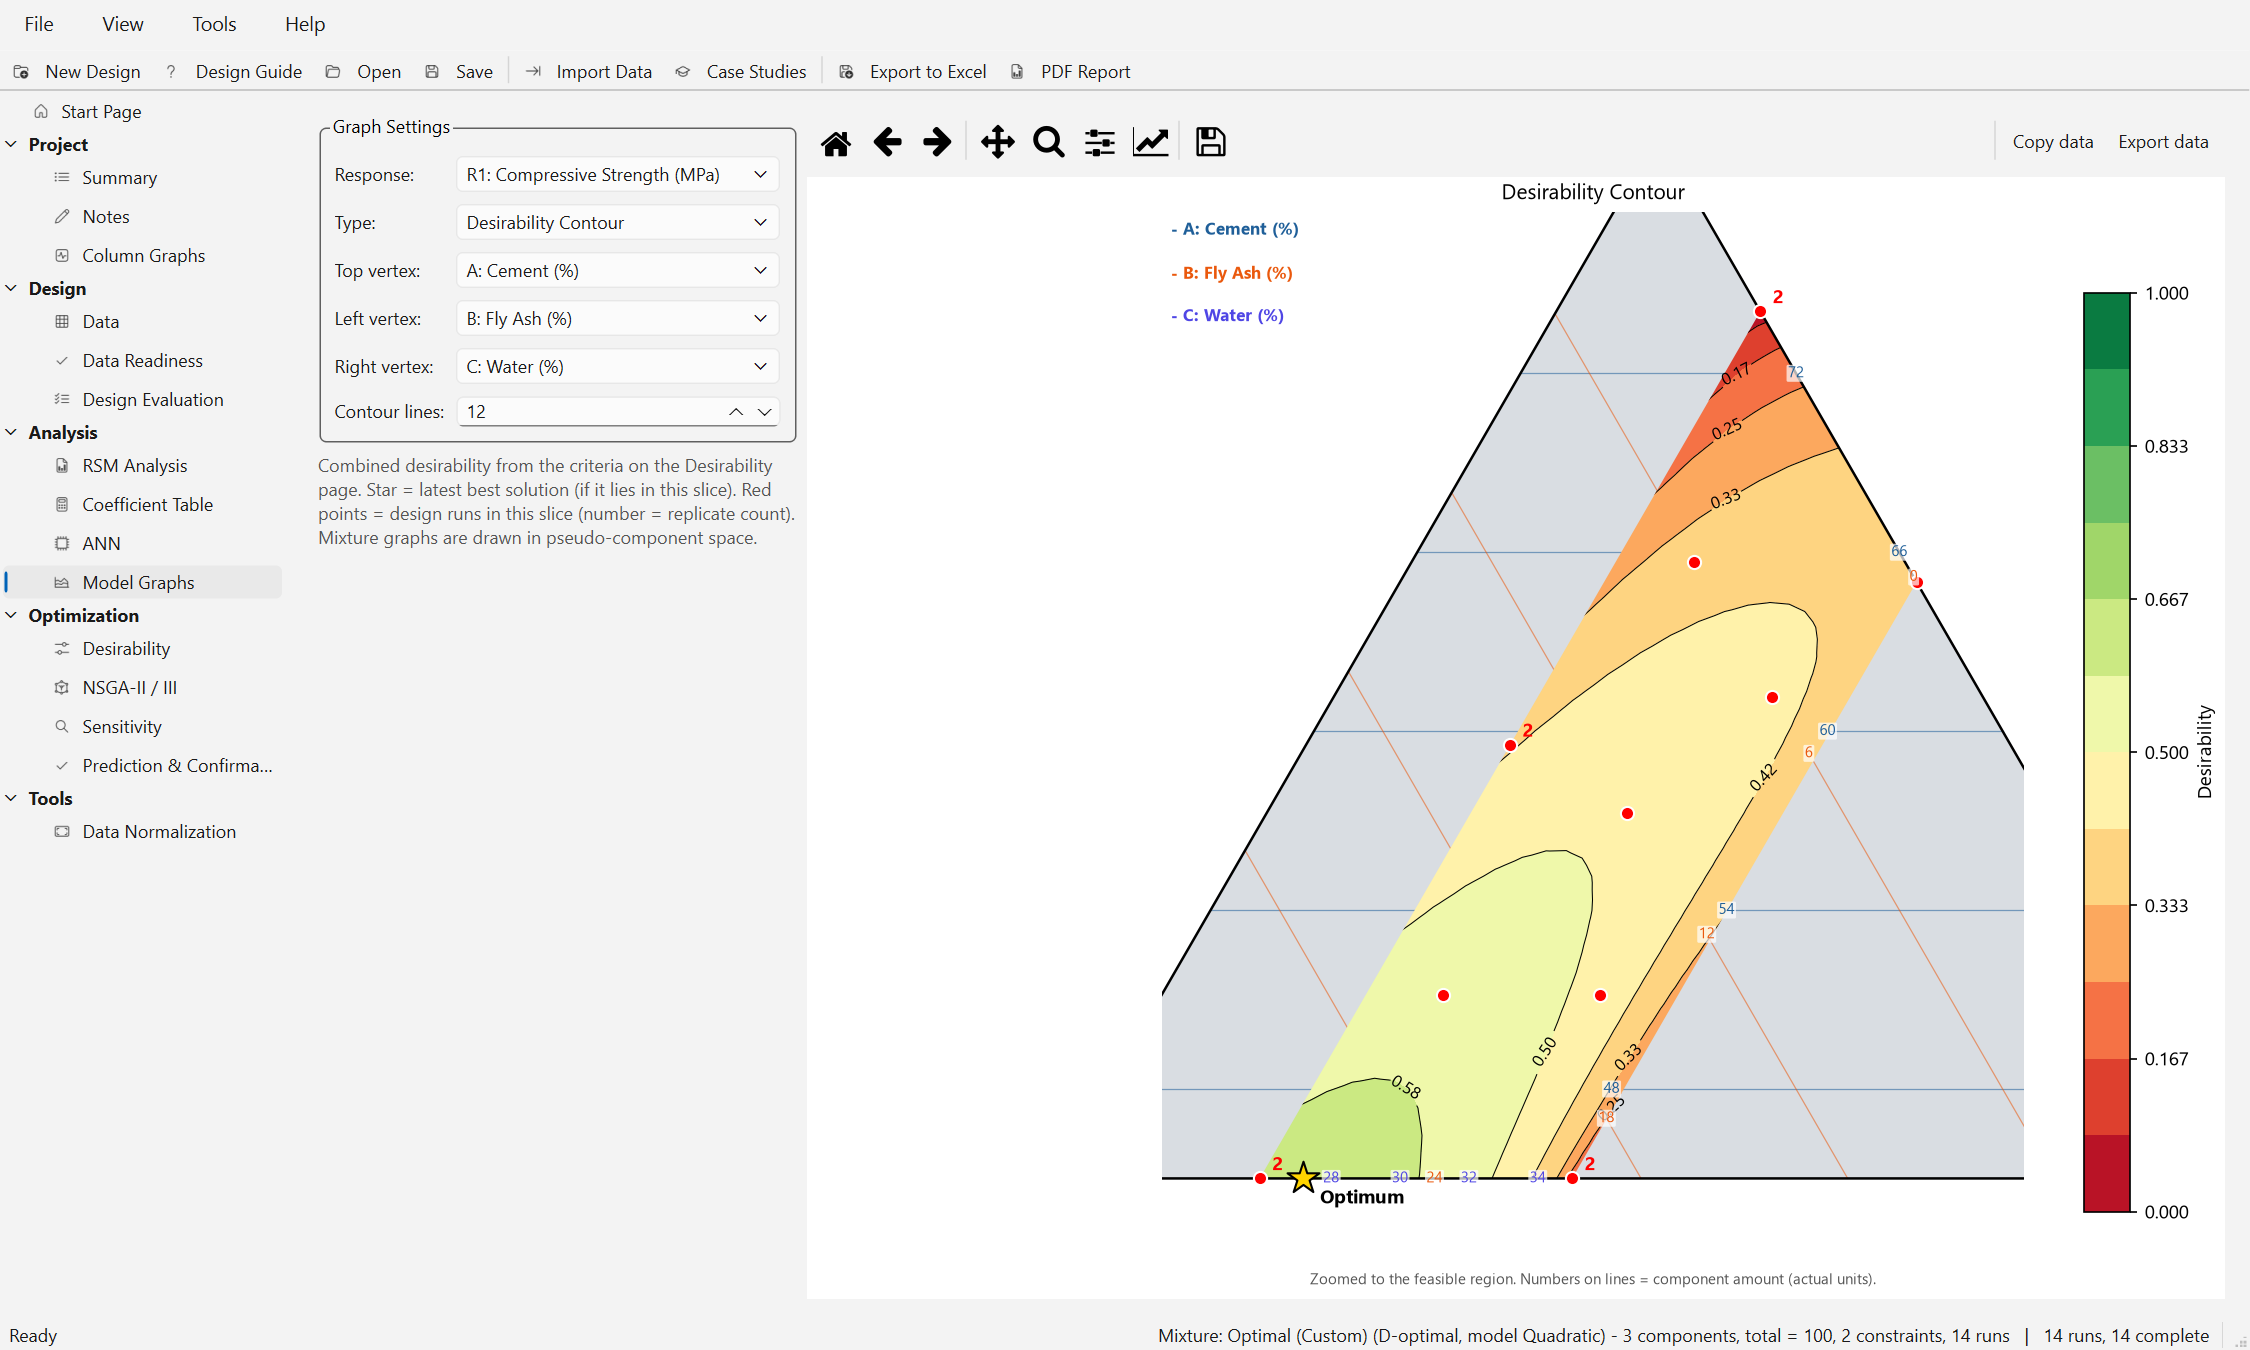
\includegraphics[width=\linewidth]{moo_concrete_desirability.png}
\caption{\ui{Desirability Contour} of the concrete mix paste in the constrained ternary region (pseudo-components,
zoomed to the feasible band between the two water/binder constraints); the star marks the best desirability blend.}
\label{fig:ch11-concrete-desir}
\end{figure}

% ======================================================================================================
\section{Checklist for the multi-objective study}
\label{sec:ch11-checklist-moo}
\begin{table}[htbp]
\centering
\small
\caption{What to report, with the values of the polygeneration example (Part C).}
\label{tab:ch11-checklist-moo}
\begin{tabularx}{\linewidth}{@{}>{\raggedright\arraybackslash}p{2.6cm} >{\raggedright\arraybackslash}X@{}}
\toprule
Item & Polygeneration plant example \\
\midrule
Data & 80 simulated runs (Latin hypercube) of an illustrative plant model, 5 decision variables; readiness \ui{Ready}
(modeling 92/92/92, optimization 91/94/91); no replicates. \\
Models & Quadratic RSM, predicted $R^2$ 0.992, 0.967, 0.990 (efficiency, cost, impact). \\
Check A & ANN 5-3-1, 5-8-4-1, 5-4-1; $Q^2$ 0.990, 0.955, 0.988 against RSM 0.992, 0.962, 0.989 on the same folds;
RSM kept. \\
Check B & ANN test $R^2$ 0.984, 0.964, 0.984 against RSM 0.991, 0.970, 0.989 with the full data. \\
NSGA & NSGA-III, population 200 (100 did not converge), seed 1, automatic stop at generation 145, 197 solutions. \\
Check C & Population 100: not converged after 300 (or 600) generations. Population 200: converged at generation 145
(gain +0.045~\% $<$ 0.19~\%, ideal point shift 0.16~\%), population check slightly above the limits (1.2~\%, 1.4~\%).
Population 400: converged at 115, population check passed (0.66~\%, 0.98~\%); TOPSIS objectives within 0.54 points of
efficiency of the population-200 choice. \\
Check D & Passed: $\Delta=3.0$~\% (cost), $dx=14.0$~\%. \\
Sensitivity & Geothermal Temperature dominant ($\beta$ $+0.73$/$-0.58$/$+0.84$; Sobol $S_T$ 0.47/0.36/0.60); sum of
$S_1\ge0.996$. \\
Compromise & TOPSIS 218.5~°C, 1401~kPa, 10.7~°C, 0.750, 50.6~°C: 20.13~\%, 18.19~USD/GJ, 3.934~mPts/h; knee as
low-impact alternative. \\
Confirmation & One plant-model evaluation; PI (95~\%, $n=1$) 19.74--20.53~\%, 17.61--18.78~USD/GJ, 3.848--4.019~mPts/h. \\
\bottomrule
\end{tabularx}
\end{table}
